\documentclass[12pt, a4paper]{extarticle}

\usepackage[utf8]{inputenc}
\usepackage[T2A]{fontenc}
\usepackage[top=2cm, bottom=1.5cm, left=1.5cm, right=1.5cm, headheight=28pt, headsep=0.5cm]{geometry}
\usepackage[english, russian]{babel}
\usepackage{tcolorbox}
\usepackage{graphicx}
\usepackage[fleqn]{amsmath}
\usepackage{amssymb}
\usepackage{hyperref}
\hypersetup{
    colorlinks=true,
    linkcolor=blue,
    urlcolor=blue,
    citecolor=red,
    pdfborder={0 0 0}
}

\usepackage{titlesec}
\usepackage{fancyhdr}
\usepackage{xcolor}
\usepackage{enumitem}
\usepackage{listings}
\usepackage{indentfirst}
\usepackage{tabularx}
\setlength{\parindent}{1cm}


\lstset{
    language=C++,
    basicstyle=\ttfamily\small,
    keywordstyle=\color{blue}\bfseries,
    commentstyle=\color{green!50!black}\itshape,
    stringstyle=\color{red},
    numbers=left,
    numberstyle=\tiny\color{gray},
    stepnumber=1,
    numbersep=5pt,
    backgroundcolor=\color{gray!10},
    frame=single,
    rulecolor=\color{black!30},
    tabsize=4,
    breaklines=true,
    captionpos=b
}

\DeclareMathOperator{\Ln}{Ln}
\DeclareMathOperator{\im}{Im}
\DeclareMathOperator{\re}{Re}
\DeclareMathOperator{\res}{res}

\titleformat{\section}{\normalfont\large\bfseries}{}{0cm}{}
\titleformat{\subsection}{\normalfont\normalsize\bfseries}{}{0cm}{}

\pagestyle{fancy}
\fancyhf{} % очистка
\fancyhead[L]{\color{gray!70}\nouppercase{\leftmark}}
\fancyfoot[R]{\thepage}

\fancypagestyle{plain}{
  \fancyhf{}
  \renewcommand{\headrulewidth}{0pt}
}

\linespread{1.25}


\newcommand{\textbfit}[1]{\textbf{\textit{#1}}}

\begin{document}

% \thispagestyle{plain}
% \title{Комплексный анализ}
% \author{Алёна Новикова \thanks{Конспект лекций Вероники Евгеньевны Владыкиной}}
% \date{2026}
% \maketitle


\begin{titlepage}
    \begin{center}
        \vspace*{3cm}
        
        {\Huge Комплексный анализ}
        
        \vspace{1cm}
        {\Large \textit{Конспект лекций}}
        
        \vspace{3cm}
        
        {\Large Алёны Новиковой}
        
        \vspace{1.5cm}
        
        {\large \text{по лекциям}} \\
        {\Large \text{Вероники Евгеньевны Владыкиной}}
        
        \vfill
        
        {\large 2026}
    \end{center}
\end{titlepage}

\newpage
\thispagestyle{plain}
\tableofcontents

\newpage

\section{Лекция 15. Комплексные числа. Операции над ними. Стереографическая проекция}\label{lection1}

\subsection{Комплексные числа. Операции над ними}

\textbfit{Опр.} Комплексное число -- пара чисел $(x, y), \ x, y \in \mathbb{R}$.

\textbfit{Обозначение:} $(1, 0) =: 1, \ (0, 1) =: i$
\[(x, y) = x \cdot 1 + y \cdot i = x + iy\]
\[(1, 0) \cdot (1, 0) = 1; \ 1 \cdot i = i \cdot 1 = i; \ i \cdot i = -1\]
\[(x_1+iy_1) \cdot (x_2+iy_2) = x_1 x_2 + iy_1 x_2 + iy_2 x_1 - y_1 y_2\]
\[z^{-1} := \frac{x}{x^2+y^2} + i \frac{-y}{x^2+y^2}\]
\[z^{-1} \cdot z = z \cdot z^{-1} = 1\]

Остальные свойства проверяются очевидно, значит, $\mathbb{C}$ -- поле.
\[\frac{z_1}{z_2} := z_1 \cdot z_2^{-1}\]

\textbfit{Опр.} Комплексным сопряжённым к числу $z = x + iy$ называется число $\overline{z} = x - iy$.

\textbfit{Опр.} Модулем числа $z = x+iy$ называется число $|z| = \sqrt{x^2+y^2}$.

\[z = |z| \left(\frac{x}{|z|} + i\frac{y}{|z|}\right) = |z|(\cos \varphi + i \sin \varphi)\]

\textbfit{Опр.} Число $\varphi$ называют аргументом числа $z$, если $\begin{cases}\cos \varphi = \frac{x}{|z|} \\ \sin \varphi = \frac{y}{|z|}\end{cases}$

\textbfit{Опр.} $Arg \ z = \{\varphi \in \mathbb{R} | \varphi = \arg z\}$

Для 0 аргумент не определён.

\textbfit{Обозначение} (Эйлера): $e^{i\varphi} := \cos \varphi + i \sin \varphi$ (на данный момент считаем картинкой, не верим, что это получено из ряда Тейлора)

\textbfit{Утв.} $e^{i(\varphi_1+\varphi_2)} = e^{i\varphi_1} e^{i\varphi_2}$
\[\triangleright 
\includegraphics[width=0.3\textwidth]{очев.png}\blacktriangleleft\]

\textbfit{Утв.} (Формула Муавра) $(e^{i\varphi})^n = e^{in\varphi}$

\textbfit{Утв.} $z = |z| e^{i\varphi}$ (полярный вид числа), $\overline{z} = |z| e^{-i\varphi}$

\textbfit{Утв.} $z_1 = |z_1| e^{i\varphi_1}, \ z_2 = |z_2| e^{i\varphi_2} \Rightarrow \ z_1 z_2 = |z_1| \cdot |z_2| e^{i(\varphi_1+\varphi_2)}, \ \frac{z_1}{z_2} = \frac{|z_1|}{|z_2|} e^{i(\varphi_1-\varphi_2)}$
\[\triangleright \ z_2^{-1} = \frac{x_2}{x_2^2+y_2^2} - i \frac{y_2}{x_2^2+y_2^2} =\frac{1}{|z_2|^2} \overline{z_2} = \frac{1}{|z_2|^2} \cdot |z_2| e^{-i\varphi_2} \blacktriangleleft\]
\[z^n = |z|^n e^{in\varphi}\]

\textbfit{Утв.} $z_1 = z_2 \Leftrightarrow \begin{cases} |z_1|=|z_2| \\ Arg \ z_1 = Arg \ z_2\end{cases}$

\textbfit{Опр.} $\sqrt[n]{z}, \ n \in \mathbb{N}$ называется число $w \in \mathbb{C} : w^n = z$ (любое из подходящих чисел).
\[w = |w| e^{i \arg (w)}\]
\[w^n = |w|^n e^{in \arg (w)} = |z| e^{i \arg (z)}\]
\[|w|^n = |z|, \ n \arg(w) = \arg(z) + 2\pi k\]
\[|w| = \underset{0}{\sqrt[n]{|z|}}, \ \arg(w) = \frac{\arg(z) + 2\pi k}{n}, \ k=0,\ldots,n-1\]

\subsection{Стереографическая проекция}

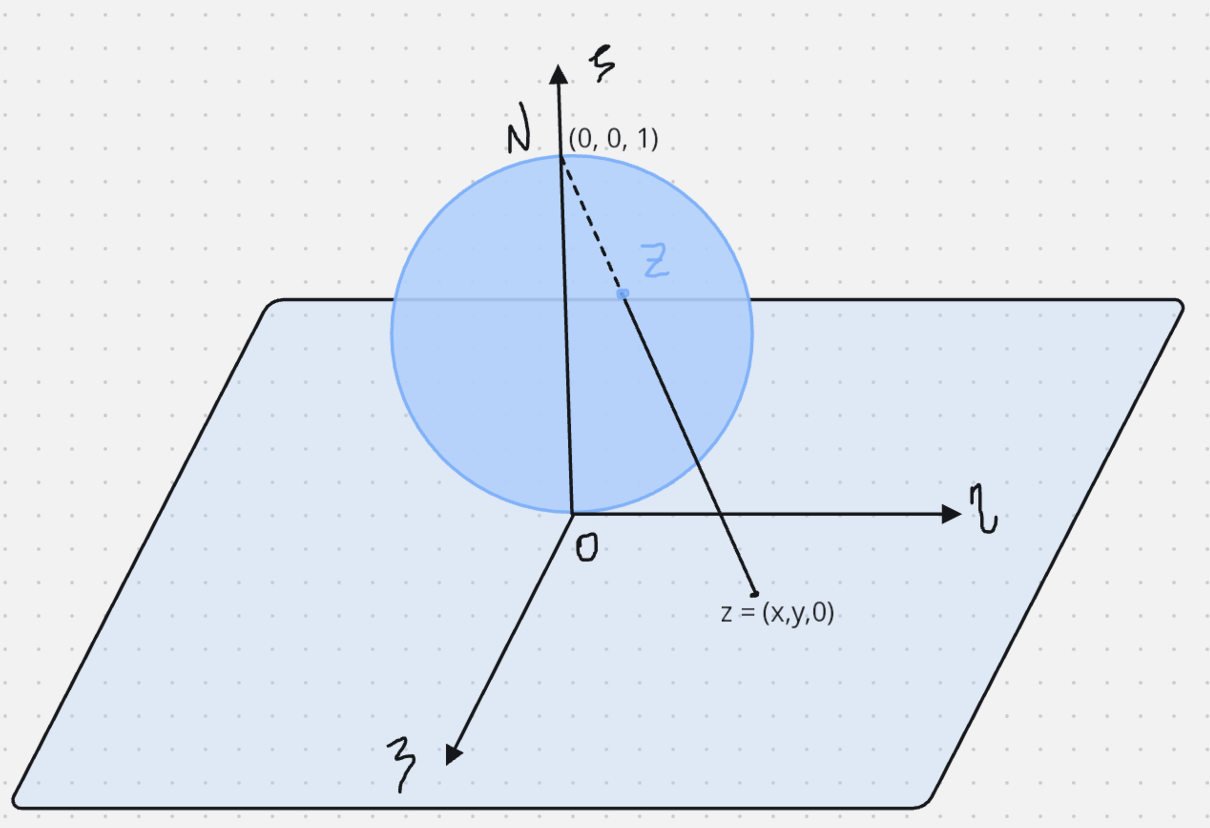
\includegraphics[width=0.6\linewidth]{Riman_sphere.png}
\[\xi^2 + \eta^2 + \left(\zeta - \frac{1}{2}\right)^2 = \frac{1}{4} \text{ -- сфера Римана}\]

\textbfit{Опр.} Стереографической проекцией называется биекция $\mathbb{C}$ и $S \setminus \{N\} : z = (x_0, y_0) \leftrightarrow Z = S \cap zN$
\[N(0, 0, 1) \text{ -- полюс}, \ \overline{a} = (x, y - 1)\]
\[Nz : \begin{cases} \xi = xt \\ \eta = yt \\ \zeta = 1 - t \end{cases}\]
\[x^2t^2 +y^2t^2 + \left(\frac{1}{2} - t\right)^2 = \frac{1}{4}\]
\[t^2(|z|^2+1) = t\]
\[t = \frac{1}{|z|^2+1}\]
\[\begin{cases}
    \xi = \frac{x}{|z|^2+1} \\
    \eta = \frac{y}{|z|^2+1} \\
    \zeta = 1 - \frac{1}{|z|^2+1} = \frac{|z|^2}{|z|^2+1}
\end{cases}\]

Обратно $Z(\xi, \eta, \zeta) \rightarrow z$
\[t = 1 - \zeta, \ x = \frac{\xi}{1-\zeta}, \ y = \frac{\eta}{1-\zeta}\]

\textbfit{Опр.} Говорят, что $z_n \to \infty$, если $|z_n| \to \infty$

\textbfit{Опр.} $\overline{\mathbb{C}} = \mathbb{C} \cup \{\infty\}$ -- расширение комплексной плоскости.

\textbfit{Опр.} Доопределим стереографическую проекцию $\infty \leftrightarrow N$, т.о. это биекция $S$ и $\overline{\mathbb{C}}$.

\textbfit{Опр.} Сферическим расстоянием между $z_1, z_2 \in \overline{\mathbb{C}}$ называется расстояние между их стереографическими проекциями.
\[\rho(z_1, z_2) = |Z_1-Z_2|\]

\textbfit{Утв.} $z_1, z_2 \in \mathbb{C}, \ \rho(z_1, z_2) = \frac{|z_1-z_2|}{\sqrt{1+|z_1|^2}\sqrt{1+|z_2|^2}}, \ \rho(z, \infty) = \frac{1}{\sqrt{1+|z|^2}}$.
\[\triangleright \ \left(\xi, \eta, \zeta\right)\]
\[\rho^2(z_1, z_2) = \left(\frac{x_1}{1+|z_1|^2}-\frac{x_2}{|z_2|^2+1}\right)^2 + \left(\frac{y_1}{1+|z_1|^2} - \frac{y_2}{1+|z_2|^2}\right)^2 + \left(\frac{|z_1|^2}{1+|z_1|^2} - \frac{|z_2|^2}{1+|z_2|^2}\right)^2 =\]
\[=  \ldots = \frac{(x_1-x_2)^2 + (y_1-y_2)^2}{(1+|z_1|^2)(1+|z_2|^2)} \ \blacktriangleleft\]

\textbfit{Утв.} Пусть $|z| \geq R$. Тогда $Z=(\xi, \eta, \zeta) : \zeta \in \left[\frac{R^2}{1+R^2}, 1\right]$.

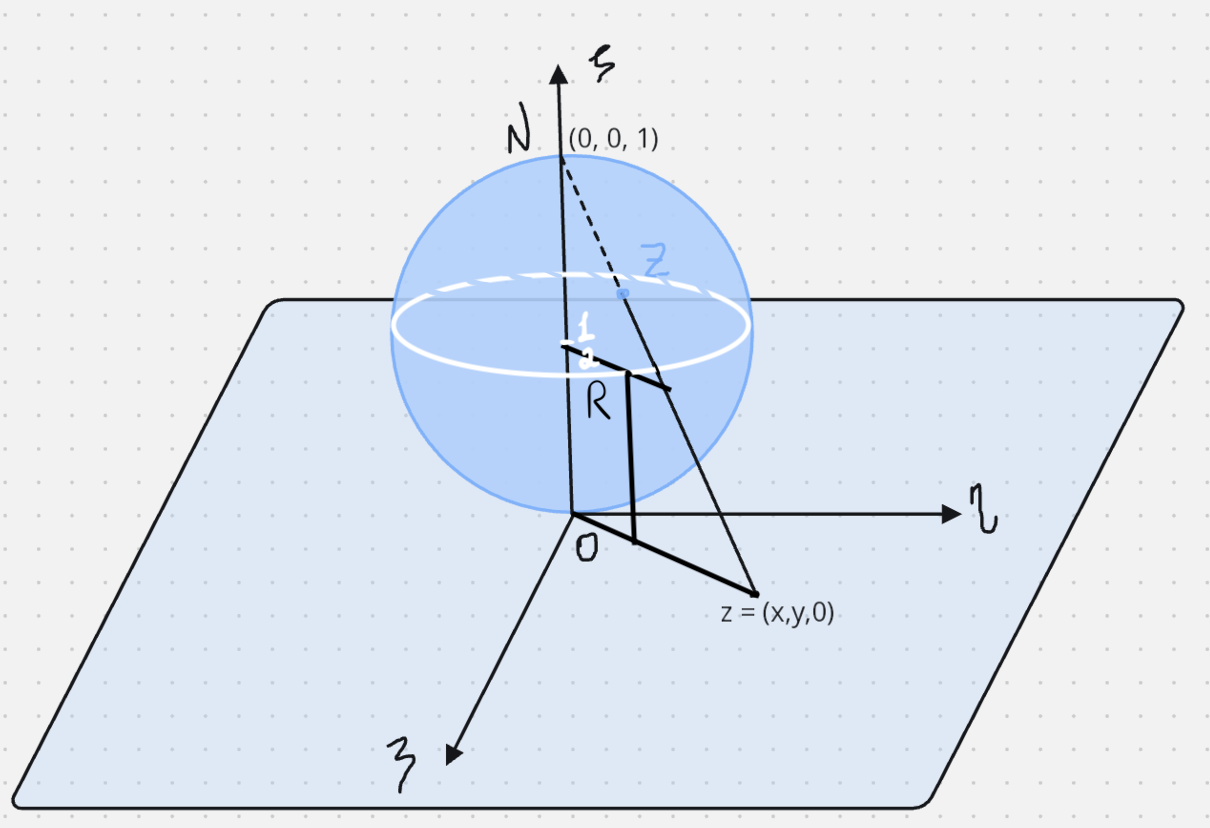
\includegraphics[width=0.6\linewidth]{Riman_sphere_2.png}
\[ \triangleright \ |z| = R\]
\[(\xi, \eta, \zeta) = \left(\frac{x}{|z|^2+1}, \frac{y}{|z|^2+1}, \frac{R^2}{R^2+1}\right)\]
\[\xi^2 + \eta^2 = \frac{x^2+y^2}{(|z|^2+1)^2} = \frac{R^2}{(R^2+1)^2}, \text{ т.е. образ точек такого вида -- окружность } r = \frac{R}{R^2+1}\]
\[\zeta = 1 - \frac{1}{1+R^2} \uparrow |z| \to \infty \ \blacktriangleleft\]


\section{Лекция 2. Экспонента}
\textbfit{Утв.} Сходимость в $\overline{\mathbb{C}}$ равносильна сходимости по сферической метрике.
\[\triangleright \ 1) z \in \mathbb{C}\]
\[(\Rightarrow) \text{ Пусть } z_n \in \mathbb{C}, \ z_n \to z \in \mathbb{C}\]
\[\rho(z_n, z) = \frac{|z_n-z|}{\sqrt{1+|z_n|^2}\sqrt{1+|z|^2}} \leq |z_n-z|\to 0\]
\[(\Leftarrow) \text{ Пусть } \rho(z_n, z) \to 0, z \in \mathbb{C}\]
\[(\xi_n, \eta_n, \zeta_n)\to(\xi, \eta, \zeta) \Rightarrow \zeta_n\to \zeta\]
\[\zeta < 1 \Rightarrow \exists N: \forall n > N \ \zeta_n < R_0 < 1 \Rightarrow \exists R: \forall n > N \ |z_n| < R, |z| < R\]
\[0 \leftarrow \rho(z_n, z) = \frac{|z_n-z|}{\sqrt{1+|z_n|^2}\sqrt{1+|z|^2}} \geq \frac{|z_n-z|}{1+R^2}, \ \text{т.к. } |z_n| < R, \ |z| < R\]
\[2) z = \infty \in \overline{\mathbb{C}}\]
\[(\Rightarrow) \text{ Пусть } z_n \to z = \infty \text{ в } \overline{\mathbb{C}}\]
\[\rho(z_n, z) = \frac{1}{\sqrt{1+|z_n|^2}} \to 0\]
\[(\Leftarrow) \ \rho(z_n, \infty) \to 0 \Rightarrow \frac{1}{\sqrt{1+|z_n|^2}} \to 0 \Rightarrow \sqrt{1+|z_n|^2} \to \infty \Leftrightarrow |z_n| \to \infty \blacktriangleleft\]

Говорят, что $\overline{\mathbb{C}}$ и $S$ -- \textit{компактификация} $\mathbb{C}$.

\textbfit{Утв.} $z_n = x_n +iy_n, \ z=x+iy, \ z_n = r_n e^{i\varphi_n}, \ z=re^{i\varphi}, \ r_n>0, \ r>0$

1) $z_n \to z \Leftrightarrow \begin{cases}
x_n \to x \\
y_n \to y   
\end{cases}$

2) $z_n \to 0 \Leftrightarrow r_n \to 0$ 

3) $r_n \to r, \ \varphi_n \to \varphi \Rightarrow z_n \to z$

4) $z_n \to z, \ z \neq 0 \Rightarrow r_n \to r, \ \exists \varphi_n = \arg z_n, \ \exists \varphi = \arg z: \varphi_n \to \varphi$
\[\triangleright \ (1)-(2) \text{ очевидно}\]
\[(3): \ z_n = r_n (\cos \varphi_n + i\sin \varphi_n)\] 
\[x_n = r_n \cos \varphi_n \to r\cos \varphi, \ y_n = r_n \sin \varphi_n \to r\sin \varphi \overset{(1)}{\Rightarrow} z_n \to z\]
\[(4): |z_n-z|\to 0, \ |z_n-|z|| \leq |z_n-z|\to 0\]
\[z \neq 0\]
\[\text{1) Пусть } x > 0, x_n\to x \Rightarrow x_n > 0 \ n > N \Rightarrow \text{(они в правой полуплоскости) можно выбрать } \]
\[\arg z_n \in \left(-\frac{\pi}{2}, \frac{\pi}{2}\right), \ \varphi_n = \arctg \frac{y_n}{x_n} \to \arctg \frac{y}{x} \in Arg(z)\]
\[\text{Остальное аналогично.} \ \blacktriangleleft\]

\subsection{Экспонента}
\textbfit{Опр.} $e^z := \lim_{n\to\infty} \left(1+\frac{z}{n}\right)^n$

\textbfit{Утв.} Определение корректно, предел существует, причём $e^{z} = e^x e^{iy} = e^x(\cos y + i\sin y)$
\[\triangleright \left(1+\frac{z}{n}\right)^n = \left(1+\frac{x}{n} + i\frac{y}{n}\right)^n\]
\[\left|\left(1+\frac{x}{n}+i\frac{y}{n}\right)^n\right| = \left|1+\frac{x}{n}+i\frac{y}{n}\right|^n = \left(\left(1+\frac{x}{n}\right)^2+\frac{y^2}{n^2}\right)^\frac{n}{2} = \left(1+\frac{2x}{n} + \frac{x^2+y^2}{n^2}\right)^\frac{n}{2} =\]
\[= e^{\frac{n}{2}\ln\left(1+\frac{2x}{n}+\frac{x^2+y^2}{n^2}\right)} = e^{\frac{n}{2}\left(\frac{2x}{n}+o\left(\frac{1}{n}\right)\right)} \to e^x\]
\[1+\frac{x}{n} \text{ начиная с какого-то номера лежит в правой полуплоскости}\]
\[\varphi_n = \arg\left(1+\frac{x}{n} + i\frac{y}{n}\right) = \arctg \frac{\frac{y}{n}}{1+\frac{x}{n}} = \arctg \frac{y}{n+x}\]
\[\arg \left(1+\frac{x}{n}+i\frac{y}{n}\right)^n = n \cdot \varphi_n = n\arctg \frac{y}{n+x} = n\left(\frac{y}{n+x} + o\left(\frac{1}{n}\right)\right) \to y \blacktriangleleft\]

\textbfit{Сл.} 1) $e^{z_1+z_2} = e^{z_1}\cdot e^{z_2}$

2) $e^{z+2\pi i} = e^z e^{2\pi i} = e^z$

\textbfit{Опр.} $\cos z := \frac{e^{iz}+e^{-iz}}{2}$

$\sin z := \frac{e^{iz}-e^{-iz}}{2i}$

$\tg z := \frac{\sin z}{\cos z}$

$\ctg z := \frac{\cos z}{\sin z}$

$\ch z := \frac{e^z+e^{-z}}{2}$

$\sh z := \frac{e^z-e^{-z}}{2}$

\textbfit{Утв.} $\ch z = \cos (iz)$

$\sh z = -i\sin(iz)$

$\ch^2 z - \sh^2z = 1$

\textbfit{Опр.} Пусть $z \neq 0$. Тогда $\Ln z$ называется число $w \in \mathbb{C}: e^w = z$

\textbfit{Утв.} Если $z = re^{i\varphi}\neq 0$, то $\Ln z = \ln r + i\varphi + 2\pi i k, k \in \mathbb{Z}$ 
\[\triangleright \ w = u+iv, \ e^w = e^u e^{iv} = re^{i\varphi} = z \Leftrightarrow e^u = r, \ v = \varphi +2\pi k, k \in \mathbb{Z} \blacktriangleleft\]

\textbfit{Опр.} $z^w := e^{w\Ln z}, z \neq 0$

\textbfit{Утв.} $z^n = \prod_{i=1}^n z, \ z^{\frac{1}{n}} = \sqrt[n]{z}$
\[\triangleright \ 1)\ z^n = e^{n \ln z} = e^{n(\ln|z|+i\varphi+2\pi i k)} = e^{n\ln |z|}e^{in\varphi}e^{i2\pi kn} = \prod_{i=1}^n z\]
\[2)\ e^{\frac{1}{n}}=e^{\frac{1}{n} (\ln |z| + i\varphi + 2\pi ik)} = e^{\frac{1}{n}\ln|z|}e^{i\frac{\varphi+2\pi k}{n}} = \sqrt[n]{z}, \ k \in \mathbb{Z} \blacktriangleleft\]

$A\cdot z = |A| e^{i\arg A}|z|e^{i\arg z}$

$f: \mathbb{R}^2\to\mathbb{R}^2$
\[f(z) = |A|\left(\begin{array}{ll}\cos \varphi & -\sin \varphi \\
\sin \varphi & \cos \varphi \end{array}\right)\left(\begin{array}{ll} x \\ y    
\end{array}\right), \ \varphi = \arg A\]

\textbfit{Опр.} Пусть $f: \mathbb{C}\to\mathbb{C} \ (\mathbb{R}^2\to \mathbb{R}^2)$

$f(z) =f(x, y) = \left(\begin{array}{ll} u(x, y) \\ v(x, y) \end{array}\right) = u(x, y) + iv(x,y)$

Говорят, что $f \ \mathbb{R}$-дифференцируема, если она дифференцируема, как функция из $\mathbb{R}^2\to\mathbb{R}^2$, т.е. $u, v$ -- дифференцируемые функции.
\[\left(\begin{array}{ll}u(x_0+\Delta x, y_0+\Delta y)-u(x_0,y_0)\\ v(x_0+\Delta x, y_0 + \Delta y) - v(x_0, y_0)\end{array}\right) = \left(\begin{array}{ll}
A & B \\ C & D
\end{array}\right) \left(\begin{array}{ll}
\Delta x \\ \Delta y    
\end{array}\right) + o(|\Delta z|) \] 
\[A=u_x(x_0, y_0), B = u_y(x_0, y_0), C = v_x(x_0, y_0), D = v_y(x_0, y_0)\]
\[f(z_0+\Delta z)-f(z_0)=A\Delta x+B\Delta y + i(C\Delta x + D\Delta y)+o(\Delta z) = (*)\]
\[\Delta x = \frac{\Delta z + \Delta \overline{z}}{2}, \ \Delta y = \frac{\Delta z - \Delta \overline{z}}{2i}\]
\[(*) = \frac{\Delta z}{2}(A -iB+iC+D)+\frac{\Delta \overline{z}}{2}(A+iB+iC-D) + o(\Delta z)\]
\[\frac{\partial f}{\partial z} = \frac{A -iB+iC+D}{2}\]
\[\frac{\partial f}{\partial \overline{z}} = \frac{A+iB+iC-D}{2}\]

\textbfit{Опр.} Пусть $f:\mathbb{C}\to\mathbb{C}$. Говорят, что $f \ \mathbb{C}$--дифференцируема, если $\exists \lim_{\Delta z\to 0} \frac{f(z_0+\Delta z)-f(z_0)}{\Delta z} =: f'(z_0)$


\section{Лекция 3. Условия Коши-Римана. Голоморфность}
\subsection{Условие Коши-Римана}

\textbfit{Теорема} (Коши-Римана) Пусть $f:U(z_0) \to \mathbb{C}. \ f - \mathbb{C}-$дифференцируема в $z_0 \Leftrightarrow \mathbb{R}-$диф-

ференцируема в $z_0$ и выполнено условие Коши-Римана $\begin{cases}
    u_x = v_y \\
    u_y = -v_x
\end{cases}$, т.е. $\frac{\delta f}{\delta \overline{z}}=0$
\[\triangleright (\Rightarrow) f(z_0+\Delta z)-f(z_0)=f'(z_0)\Delta z +\overline{o}(\Delta z) = |f'(z_0)|\left(\begin{array}{ll}
\cos \phi & -\sin \phi \\
\sin \phi & \cos \phi    
\end{array}\right) \left(\begin{array}{ll}
 \Delta x \\
 \Delta y   
\end{array}\right) + \overline{o}(|\Delta z|)\]
\[\Rightarrow u_x = |f'(z_0)|\cdot \cos \phi \ldots \Rightarrow \text{Коши-Римана выполнено, и $f \ \mathbb{R}-$дифференцируема}\]
\[(\Leftarrow) f(z_0+\Delta z)-f(z_0) = \frac{\delta f}{\delta z} \Delta z + \frac{\delta f}{\delta z} \Delta \overline{z}+\overline{o}(\Delta z) = \frac{\delta f}{\delta z}\Delta z + \overline{o}(\Delta z) \Rightarrow\]
\[\Rightarrow f \ \mathbb{C}-\text{дифференцируема и } f'(z_0) = \frac{\delta f}{\delta z}\Big|_{z_0} \blacktriangleleft\]

\textbfit{Пр.} $f(z) = \overline{z} = x-iy$
\[u(x, y) = x, \ v(x, y) = -y\]
\[\begin{cases}
    1 \neq -1 \\
    0 = 0
\end{cases}\]
\[\frac{\delta f}{\delta \overline{z}} = 1 \neq 0\]
\[\text{Условие Коши-Римана не выполнено, значит, не $\mathbb{C}-$дифференцируема.}\]
\textbfit{Опр.} Пусть $\theta \in \mathbb{R}, \ f:U(z_0)\to\mathbb{C}$. Тогда производной по направлению $\theta$ называется $f'_\theta(z_0) = \lim_{\Delta z \to 0, \ \arg \Delta z = \theta} \frac{f(z_0+\Delta z)-f(z_0)}{\Delta z}$
\[f'_0(z_0) = u_x +iv_x\]
\[f'_{\frac{\pi}{2}} = -i(u_y+iv_y)\]
\textbfit{Опр.} Пусть $f-\mathbb{R}-$дифференцируема. Тогда $f-\mathbb{C}-$дифференцируема в $z_0 \Leftrightarrow f'_\theta(z_0)$ не зависит от $\theta$.
\[(\Rightarrow) \text{ очевидно}\]
\[(\Leftarrow) \Delta f = \frac{\delta f}{\delta z}\Delta z. +\frac{\delta f}{\delta \overline{z}}\Delta \overline{z}+\overline{o}(\Delta z) = (1)\]
\[\arg \Delta z = \theta, \ \Delta z = te^{i\theta}\]
\[\Delta \overline{z} = \Delta z e^{-2i\theta}\]
\[(1) = \Delta z \left(\frac{\delta f}{\delta z} + e^{-2i\theta} \frac{\delta f}{\delta \overline{z}}\right)+\overline{o}(\Delta z)=\Delta z f'_\theta (z_0) +\overline{o}(\Delta z)\]
\[\text{Но $f'_\theta$ не зависит от $\theta \Rightarrow f'_0=f''_\frac{\pi}{2}$}\]
\[\frac{\delta f}{\delta z} + \frac{\delta f}{\delta \overline{z}}=\frac{\delta f}{\delta z} -\frac{\delta f}{\delta \overline{z}}\]
\[\Rightarrow \frac{\delta f}{\delta \overline{z}} = 0 \text{, т.е. Коши-Римана.}\]
\textbfit{Пр.} 1) $z=x+iy$
\[\left(\begin{array}{ll}
1 & 0 \\
0 & 1    
\end{array}\right)\]
Условие Коши-Римана выполнено.
\[(z)'=u_x+iv_x=1\]
\[2) \ (z^n)'=nz^{n-1}\]
\[3) \ e^z = e^x(\cos y + i\sin y)\]
\[\left(\begin{array}{ll}
e^x\cos y & -e^x \sin y \\
e^x \sin y & e^x \cos y    
\end{array}\right)\]
Условие Коши-Римана выполнено.
\[(e^z)' = e^x \cos y + ie^x \sin y =e^z\]
\textbfit{Утв.} Пусть $f \in C^1 (U(z_0)), \ f'(z_0) \neq 0, \ f(z_0) = w_0$. Тогда $\exists g: U(w_0)\to U(z_0), g=f^{-1}, g \in C^1(U(w_0)), \ g-\mathbb{C}-$дифференцируема в $w_0$ и $g'(w_0)=\frac{1}{f'(z_0)}$
\[\triangleright f'(z_0) \neq 0 \Rightarrow |f'(z_0)|\neq 0, \ \arg f'(z_0) \text{ определён} ,|J| = |f'(z_0)|\neq 0\]
\[\text{Следовательно, выполнено условие теоремы об обратном отображении. }\]
\[\Rightarrow \exists g : U(w_0)\to U(z_0), \ g \in C^1, \text{ т.е. } \mathbb{R}-\text{дифференцируема и }dg\Big|_{w_0} = (df\Big|_{z_0})^{-1} =\] 
\[\left(|f'(z_0)| \left(\begin{array}{ll}
\cos \phi & -\sin \phi \\
\sin \phi & \cos \phi   
\end{array}\right)\right)^{-1} = \frac{1}{|f'(z_0)|} \left(\begin{array}{ll}
\cos \phi & -\sin \phi \\
\sin \phi & \cos \phi   
\end{array}\right) \text{ т.е. выполнено Коши-Римана}\]
\[g'(w_0) = \frac{1}{f'(z_0)} \blacktriangleleft\]
\textbfit{Пр.} $f(z) = z^2$
\[f'\Big|_{-1} = 2z=-2\]
\begin{center}
    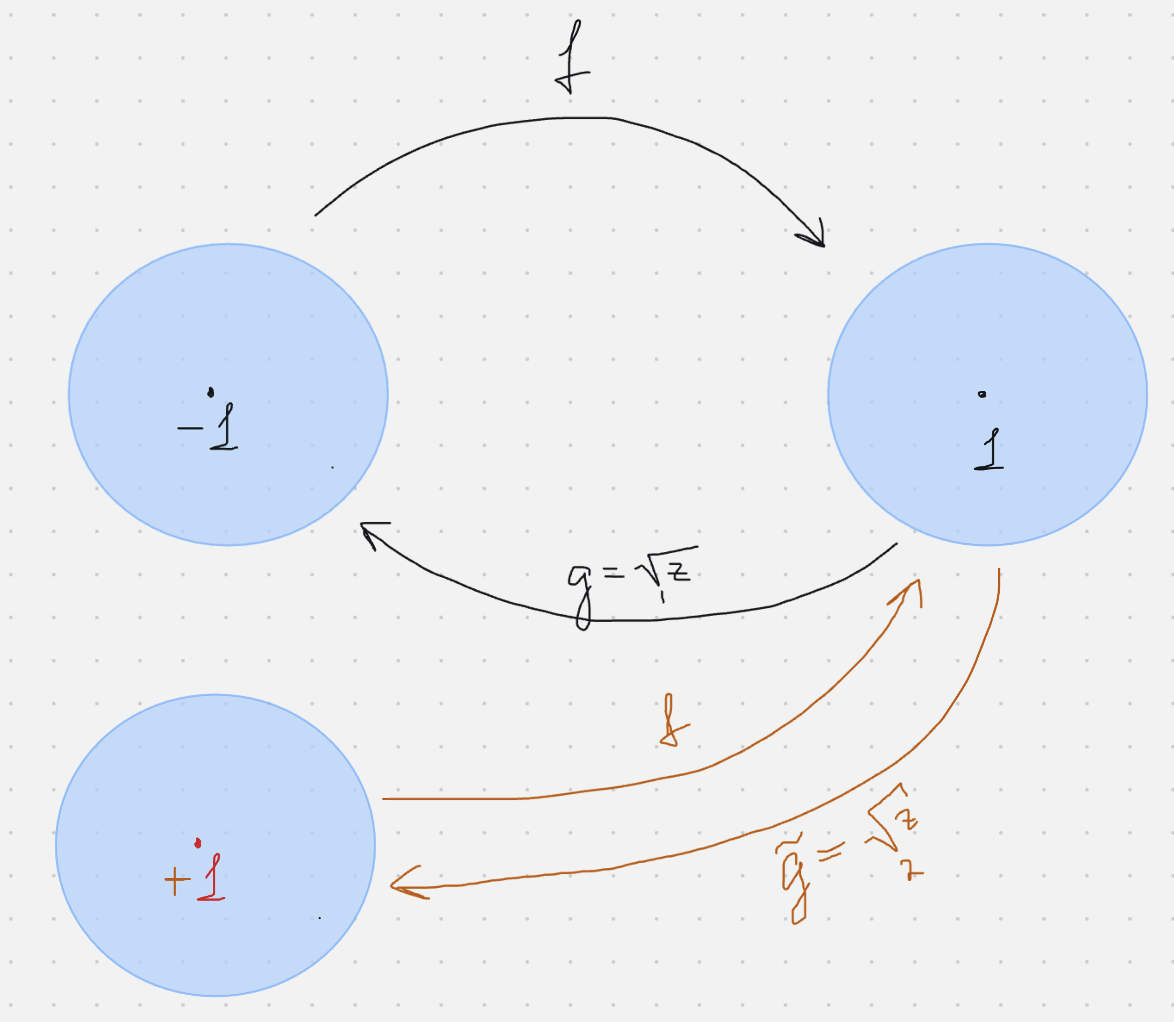
\includegraphics[width=0.5\linewidth]{lection3_1.png}
\end{center}
\[g(1) = \frac{1}{f'(-1)} = -\frac{1}{2} = \frac{1}{2\sqrt{z}_1}\]
\[g(1)=\frac{1}{f'(1)} = \frac{1}{2} = \frac{1}{2\sqrt{z}_2}\]
\textbfit{Пр.} $f(z)=e^z, \ f'(z) =e^z$
\begin{center}
    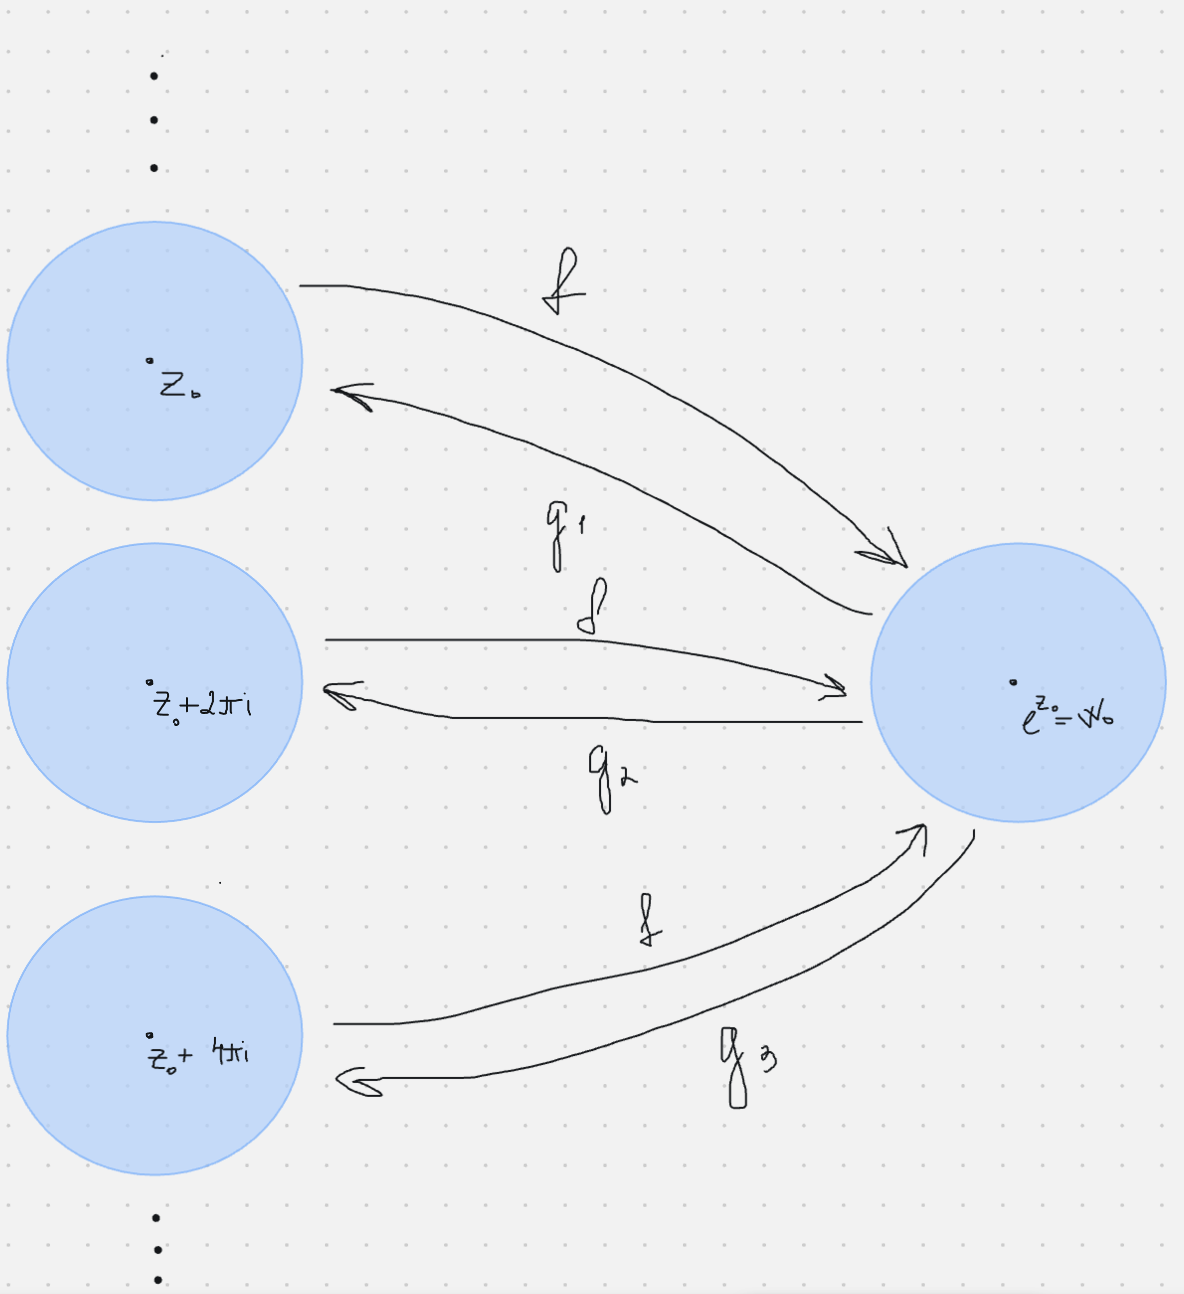
\includegraphics[width=0.5\linewidth]{lection3_2.png}
\end{center}
\[g_1(w_0)=g_1(e^{z_0})=\frac{1}{f'(z_0)}=\frac{1}{e^{z_0}}=\frac{1}{w_0}\]
\[g_i(w_0)=g_1(e^{z_0})=\frac{1}{f'(z_0+2i\pi k)}=\frac{1}{e^{z_0+2i\pi k}}=\frac{1}{w_0}\]

\textbfit{Опр.} Пусть $f: U(z_0)\to \mathbb{C}. \ f$ называется голоморфной в точке $z_0$, если $\exists U_\epsilon(z_0)$, т.ч. $f-\mathbb{C}-$дифференцируема в $U_\epsilon(z_0)$.

Если $f: D \to \mathbb{C}, \ D-$область, то говорят, что $f$ голоморфна в $D$, если она голоморфна в каждой точке $D$. Обозначение $f \in O(D)$

\textbfit{Опр.} Пусть $f:U(\infty)\to \mathbb{C}$. Говорят, что $f \ \mathbb{C}-$ дифференцируема (голоморфна), если $\mathbb{C}-$дифференцируема (голоморфна) в точке $z=0$ функция $F(z) = \begin{cases}
    f(\frac{1}{z}) \\
    f(\infty)
\end{cases}$

\textbfit{Пр.} $f(z) = \begin{cases}
    \frac{1}{z} \\ 0 & z =\infty
\end{cases}$
\[F(z) = \begin{cases}
    z \\ 0 & z = 0
\end{cases}\]

\textbfit{Опр.} Пусть $z_0 \in \overline{\mathbb{C}}, \ f:U(z_0)\to\mathbb{C}, \ f(z_0)=\infty$. Тогда она $\mathbb{C}-$дифференцируема (голоморфна) в $z_0$, если в $z_0$ голоморфна $\frac{1}{z_0}$, т.е. если $f(\infty)=\infty$, то надо изучать $\frac{1}{f(\frac{1}{z})}$ в $z=0$


\section{Лекция 4. Пути. Конформные отображения}
\subsection{Пути}
\textbfit{Опр.} Путём называется отображения $\Gamma : [a, b] \to \mathbb{C}, \ \Gamma \in C[a, b]$.
\[\Gamma(t) = x(t) +iy(t) = \left(\begin{array}{ll}
    x(t) \\
    y(t)    
\end{array}\right)\]
\[\Gamma(a) \text{ - начало пути}, \ \Gamma(b) \text{ - конец пути. Путь называется замкнутым, если } \Gamma(a) = \Gamma(b)\]

\textbfit{Опр.} Путь называется простым (жордановым), если $\Gamma-$инъекция $[a, b]$. Замкнутый путь называется жордановым, если $\Gamma-$ инъекция $[a, b].$ 

\textbfit{Опр.} Несобственным путём называется $\Gamma : [a, b] \to S, \ \Gamma \in C[a,b].$

\textbfit{Опр.} Путь $\Gamma:[a, b]\to \mathbb{C}$ называется гладким, если $\Gamma \in C^1[a,b]$ и $\overset{.}{\Gamma} \neq 0$, т.е. $\left(\begin{array}{ll}
    \overset{.}{x(t)} \\
    \overset{.}{y(t)}    
\end{array}\right) \neq \left(\begin{array}{ll}
 0 \\
 0    
\end{array}\right)$

\textbfit{Пр.} $t \in [0, 1]$
\[1) \ \Gamma(t) = t\]
\[\overset{.}{\Gamma}(t) = \left(\begin{array}{ll}
1 \\
0    
\end{array}\right) \neq 0\]
\[2) \ \Gamma(t) = t + it^2\]
\[\overset{.}{\Gamma}(t) = \left(\begin{array}{ll}
1 \\
2t   
\end{array}\right) \neq 0\]
\[3) \ \Gamma(t) = t^2+it^4\]
\[\overset{.}{\Gamma}(t) = \left(\begin{array}{ll}
2t \\
4t^3   
\end{array}\right) \neq 0\]
В примерах 2 и 3 пробежали одну и ту же параболу, но по-разному. Получили гладкий и негладкий пути из-за разной параметризации.

\textbfit{Опр.} Пусть $\Gamma: [a, b] \to \mathbb{C} - $ жорданов путь. Тогда $\gamma = \Gamma([a,b])$ называется жордановой кривой.

\textbfit{Пр.} $\Gamma(t) = e^{it}, \ t \in [0, 2\pi]$
\[\Gamma(t) = e^{2it}\]

Пробежали окружность: в первом примере единожды, во втором дважды. Первый путь -- жорданов, второй нет. По итогу окружность -- жорданова кривая.

\textbfit{Опр.} Если $\gamma -$ жорданова кривая, а $\Gamma:[a,b]\to \mathbb{C}-$ жорданов путь, т.ч. $\Gamma[a,b]=\gamma$, тогда говорят, что $\Gamma-$ параметризация $\gamma$.

Параметризация задаёт ориентацию (от A к B или от B к A).

+ обход замкнутой кривой по умолчанию считаем против часовой стрелки.

\textbfit{Пр.} $\Gamma(t) = t, \ t \in [0, 1]$
\[\Gamma(t) = 1-t\]

\textbfit{Опр.} Два гладких пути $\Gamma_1 : [a_1, b_1]\to \mathbb{C}$ и $\Gamma_2 : [a_2, b_2] \to \mathbb{C}$ называются эквивалентными, если $\exists g : [a_1, b_1] \to [a_2, b_2] \ g' > 0$ на $[a_1, b_1]$, т.ч. $g([a_1, b_1])=[a_2, b_2]$ и $\Gamma_2(g(t)) = \Gamma_1(t) \ t \in [a_1, b_1]$.

По сути пути, которые проходят прямую в одном и том же направлении.

\textbfit{Опр.} Путь $\Gamma:[a,b] \to \mathbb{C}$ называется кусочно-гладким, если $\exists$ разбиение $T = \{a=t_0<t_1<\ldots<t_k=b\}$, т.ч. $\Gamma|_{[t_{k-1}, t_k]}-$гладкий путь.

\textbfit{Опр.} Множество $A \subset \mathbb{C} (\overline{\mathbb{C}})$ называется линейно-связным, если $\forall z_1, z_2 \in A \exists$ путь (м.б. несобственный), т.ч. $\Gamma([a,b])\subset A, \Gamma(a) = z_1, \Gamma(b) = z_2$.

\textbfit{Опр.} Множество $A$ называется областью, если оно открыто и связно ($\Leftrightarrow$ в $\mathbb{R}^2$ открыто и линейно-связно).

\textbfit{Обозначение} Если $\gamma = \delta D, D-$область. $\gamma -$ замкнутая кривая. Тогда $\delta D^+ - $обход, при котором область остаётся слева. $\delta -$ граница.

\textbfit{Пр.} $(|z|=1)^+, \ \delta(|z|<1)^+=\delta (|z|>1)^-$

\textbfit{Опр.} Пусть $\gamma_1, \gamma_2 -$ две гладкие кривые. Тогда $\angle(\gamma_1, \gamma)2 = \angle(\overset{.}{\Gamma_1(t)}, \overset{.}{\Gamma_2(t)})$, где $\Gamma_1, \Gamma_2-$ гладкие параметризации. (в точке пересечения $z_0 = \Gamma_1(t_0) = \Gamma_2(t_0)$)

\textbfit{Опр.} Пусть $D-$область. $f:D \to \mathbb{C} (\overline{\mathbb{C}}), \ f$ называется однолистным в $D$, если оно инъективно в $D$.

\subsection{Конформные отображения}
\textbfit{Опр.} Пусть $f:U(z_0)\to \mathbb{C}$. Говорят, что $f$ конформно в т. $z_0$, если оно голоморфно в т. $z_0$ и $f'(z_0) \neq 0$.

$f:D\to \mathbb{C}, \ D \subset \mathbb{C}, D-$область. $f$ называют конформным в $D$, если оно конформно в каждой точке и однолистно.

Для $f: \overline{\mathbb{C}}\to\overline{\mathbb{C}}$ конформность доопределяется аналогично голоморфности.

\textbfit{Теорема} Пусть $\gamma_1, \gamma_2-$ гладкие кривые6 $z_0-$ т. пересечения. $f:U(z_0) \to \mathbb{C}, f-$ конформно в $z_0. \ \angle(\gamma_1, \gamma_2)=\angle(f(\gamma_1), f(\gamma_2)).$
\[\triangleright \text{Пусть $\Gamma(t) - $ гладкий путь.}\]
\[f(\Gamma(t)) \text{ - образ пути.}\]
\[\overset{.}{\Gamma(t)} = \left(\begin{array}{ll}
\overset{.}{x(t)} \\
\overset{.}{y(t)}   
\end{array}\right) \text{ - исходный касательный вектор.}\]
\[\overset{.}{f(\Gamma(t))} = df|_{z_0}\left(\begin{array}{ll}
\overset{.}{x(t)} \\
\overset{.}{y(t)}   
\end{array}\right) = |f'(z_0)|\left(\begin{array}{ll}
\cos \phi & -\sin \phi \\
\sin \phi & \cos \phi    
\end{array}\right) \left(\begin{array}{ll}
\overset{.}{x(t)} \\
\overset{.}{y(t)}   
\end{array}\right)\]
\[\text{Т.е. все касательные векторы поворачиваются на один и тот же угол } \phi = \arg f'(z_0)\]
\[f(z) = u(z) + iv(z), \ f(\Gamma(t)) + iv(\Gamma(t))\]
\[df|_{z_0} d\Gamma|_{t_0} = \left(\begin{array}{ll}
u_x & u_y \\ 
v_x & v_y    
\end{array}
\right) \left(\begin{array}{ll}
\overset{.}{x(t)} \\
\overset{.}{y(t)}   
\end{array}\right)\]

\textbfit{Пр.} $z^2$

Конформность нарушается в 0.

\textbfit{Теорема} (Жордана) (б/д) Пусть $\gamma-$ замкнутая Жорданова кривая. Тогда $\mathbb{C}\setminus \gamma = D_1 \cup D_2 -$ непересекающихся областей, т.ч. $\gamma = \delta D_1 = \delta D_2$.

Если $\gamma - $несобственная жорданова кривая на сфере $S$, то справедлив аналогичный факт.

Если $\gamma - $незамкнутая жорданова кривая, то $\mathbb{C} \setminus \gamma (S \setminus \gamma) - $область.

\textbfit{Теорема} Пусть $f: D \to \overline{\mathbb{C}}, D \subset \overline{\mathbb{C}}, \ f-$ конформно в $D$. $\delta D = \gamma, f\in C(D), f(\gamma) = \overline(\gamma), \gamma-$ жорданова кривая. $f(\gamma)=\overline\gamma-$ биекция. $\overline\gamma = \delta G, G-$область, $\exists z_0\in D: f(z_0)\in G.$ Тогда $f(D)=G$.

\section{Лекция 5. Дробно-линейные отображения (ДЛО)}

\textbfit{Теорема.} Пусть $f: D \to \overline{\mathbb{C}}, D \subset \overline{\mathbb{C}}, \ f$ конформно в $D$. $\partial D = \gamma, f\in C(\overline{D}), f(\gamma) = \tilde{\gamma}, \gamma \ -$ жорданова кривая. $f(\gamma)=\tilde\gamma \ -$ биекция. $\tilde\gamma = \partial G, G \ -$ область, $\exists z_0\in D: f(z_0)\in G.$ Тогда $f(D)=G$.
\[\triangleright \ \text{По т. Жордана, если $\tilde\gamma$ замкнута, то $\mathbb{C}\setminus \tilde\gamma = G$ -- область, $\tilde\gamma = \partial G$, если $\tilde\gamma$ не замкнута, то}\] 
\[\mathbb{C} \setminus \tilde\gamma = G \cup G_1, \ G, G_1 \text{ -- области, } \tilde\gamma = \partial G = \partial G_1.\]
\[\text{Т.к. $f$ -- диффеоморфизм, то $f(D)$ -- область} \Rightarrow f(D) \subset G.\]
\[\text{Хотим } f(D) = G. \text{ Пусть } G^* = G \setminus f(D).\]
\[\text{Пусть $G^*$ открыто. Тогда } G = f(D) \cup G^*, \ f(D), G^* \text{ открыты.}\]
\[\text{Это противоречит линейной связности } G. \text{ Пусть } w_1 \in f(D), w_2 \in G^*.\] 
\[\exists \Gamma(t) \text{ -- путь: } \Gamma(0) = w_1,\ \Gamma(1) = w_2, \ \Gamma(t) \in G \ \forall t\]
\[T = \inf \{t: \Gamma(t) \in G^*\}\]
\[\Gamma \text{ непрерывна } \Rightarrow \exists U_\delta(w_1) \subset f(D) \Rightarrow T >0.\]
\[\text{Пусть } T = T_0. \Gamma(T_0) = w_0 \in f(D) \text{ или } w_0\in G^* \Rightarrow [T_0 - \delta, T_0 + \delta] \in f(D) \text{ или } \in G^* \Rightarrow \exists T_n:\] 
\[T_n \to T_0, \Gamma(T_n) \in f(D) \text{ или } \exists T': T' < T_0, \Gamma(T') \in G^* \Rightarrow T \text{ не инфимум} \Rightarrow \nexists T \text{ -- противоре-}\] 
\[\text{чие }\Rightarrow G^* \text{ не открыто } \Rightarrow \exists w^* \in \partial f(D), w^* \in G, w^* \in G^* \Rightarrow \exists w_n\in f(D): w_n \to w^*,\] 
\[w_n = f(z_n).\]
\[\overline{\mathbb{C}} \text{ -- компакт} \Rightarrow \exists z_{n_k} \to z^* \in \overline{D}.\]
\[\text{Если } z^* \in D \Rightarrow \text{в силу непрерывности } w^* = f(z^*) \Rightarrow w^* \in f(D) \text{ -- противоречие с } w^* \in G^*.\]
\[\text{Если }z^* \in \partial D \Rightarrow f(z^*) \in \tilde\gamma = \partial G \text{ -- противоречие с } w^* \in G.\]
\[\text{Значит, } G^* = \varnothing. \blacktriangleleft\]

\textbfit{Утв.} $f(\partial^+(D)) = \partial^+ (f(D))$. (следует из т. Руше).
\subsection{ДЛО}
\textbfit{Опр.} Отображение $w(z) = \begin{cases}
    \frac{az+b}{cz+d}, & a, b, c, d \in \mathbb{C}, \ ad-bc \neq 0 \\
    \infty, & z = -\frac{d}{c} \\
    \frac{a}{c}, & z =\infty
\end{cases}.$

$w: \overline{\mathbb{C}}\to \overline{\mathbb{C}}$ называется ДЛО.

\textbfit{Утв.} $w$ -- гомеоморфизм $\overline{\mathbb{C}}$ на $\overline{\mathbb{C}}$.
\[\triangleright \text{ Очевидно, что $w^{-1}$ тоже ДЛО.} \blacktriangleleft\]

\textbfit{Утв.} $w$ -- конформное отображение в $\overline{\mathbb{C}}$.
\[\triangleright \ \text{Биективность уже известна.}\]
\[w' = \frac{a(cz+d) - c(az+b)}{(cx+d)^2} = \frac{ad-bc}{(cz+d)^2} \neq 0\]
\[-\frac{d}{c} \to \infty. \text{ Надо исследовать } \frac{1}{w} \text{ в } - \frac{d}{c}.\]
\[\frac{1}{w} = \frac{cz+d}{az+b}, \ \left(\frac{1}{w}\right)' = \frac{-(ad-bc)}{(az+b)^2} \neq 0\]
\[\infty \to \frac{a}{c}. \text{ Надо исследовать } w\left(\frac{1}{z}\right) \text{ в } 0.\]
\[w\left(\frac{1}{z}\right) = \frac{\frac{a}{z}+b}{\frac{c}{z}+d} = \frac{a+bz}{c+dz}, \ w\left(\frac{1}{z}\right)' = \frac{ad-bc}{(c+dz)^2} \neq 0 \blacktriangleleft\]

\textbfit{Утв.} ДЛО - композиция растяжения, сдвига, поворота и $\frac{1}{z}$.
\[\triangleright \text{ очев } \blacktriangleleft\]

\textbfit{Утв.} $\Lambda$ -- множество всех ДЛО образует группу относительно операции композиции.
\[\triangleright \text{ очев } \blacktriangleleft\]
\[\text{Группа ДЛО} \simeq GL(2, \mathbb{C}) / \mathbb{C}^* \simeq SL(2, \mathbb{C}) / \{\pm E\} = PSL(2, \mathbb{C}) = \text{группа Мёбиуса}\]

\textbfit{Теорема} (круговое свойство ДЛО и сохранение симметрии). Пусть $\Gamma$ -- обобщённая окружность (т.е. прямая или окружность). Тогда $\widetilde\Gamma = w(\Gamma)$ тоже обобщённая окружность. Причём, если $z_1, z_2$ симметричны относительно $\Gamma$, то их образы симметричны относительно $\widetilde\Gamma$.
\[\triangleright \ \text{Для поворотов и сдвигов очевидно.}\]
\[\text{Для $\lambda z$ очевидно для окружностей с центров в 0 и прямых, проходящих через 0.}\]
\[\lambda z = \lambda(z - z_0) + \lambda z_0 \Rightarrow \text{сдвигом получим для всех.}\]
\[\text{Рассмотрим } w = \frac{1}{z}\]
\[|z-z_0|^2=R^2 \text{ -- уравнение окружности.}\]
\[(z-z_0)(\overline{z} - \overline{z_0}) = R^2\]
\[z\overline{z} - z\overline{z_0} - z_0\overline{z}+z_0\overline{z_0}=R^2\]
\[Az\overline{z}+Bz+\overline{B}\overline{z} + C = 0, \ A, C \in \mathbb{R} \ldots (*)\]
\[Ax+By+C = 0 \text{ -- уравнение прямой.}\]
\[x = \frac{z+\overline{z}}{2}, \ y = \frac{z-\overline{z}}{2}\]
\[\frac{1}{2}(A-iB)z + \frac{1}{2}(A+iB)\overline{z}+C = 0\]
\[\text{Т.е. $\forall$ обобщённая окружность задаётся } (*).\]
\[\Gamma \text{ -- обобщённая окружность.}\]
\[w = \frac{1}{z} \Rightarrow z = \frac{1}{w} \to (*):\]
\[\frac{A}{w\overline{w}}+\frac{B}{w}+\frac{\overline{B}}{\overline{w}} + C = 0 | \cdot \overline{w}w\]
\[A+B\overline{w} + \overline{B} w+C\overline{w}w=0 \text{ -- обобщённая окружность.}\]
\[z_1, z_2 \text{ -- симметричные точки. } |z_1-z_0|=\frac{R^2}{|z_2-z_0|}\]
\[z_1-z_0 = \frac{R^2}{|z_2-z_0|} \cdot \frac{z_2-z_0}{|z_2-z_0|} = \frac{R^2}{\overline{z_2-z_0}}\]
\[(z_1-z_0)(\overline{z_2-z_0}) = R^2\]
\[\text{Т.е. уравнение получается из уравнения окружности } \Gamma \text{ заменой } z = z_1, \overline{z} = z_2.\]
\[\text{Прямые: } \re z =0, \ z+\overline{z} = 0\]
\[\text{Симметричные точки: } z_1+\overline{z_2}=0 \text{ выполняется.}\]
\[\text{Аналогично поворотом и сдвигом переведём } \re z \text{ в любую прямую.}\]
\[\text{Подставим в уравнение } (*) \ w_1=\frac{1}{z_1}, w_2=\frac{1}{z_2} \text{ и получим, что образы симметричны.} \blacktriangleleft\]
\section{Лекция 7. Лемма Гурса. ИТК}
\subsection{Лемма Гурса}
\textbfit{Лемма Гурса.} Пусть $f: \mathbb{C} \to \mathbb{C},\  D \ -$ область, $f \in \mathcal{O}(D)$. Тогда $\forall$ треугольника $\Delta$, т.ч. замыкание $\overline{\Delta} \subset D \ \int_{\partial \Delta}f(z) dz = 0$.
\[\triangleright \text{ От противного. Пусть } \exists \Delta_0 : \left|\int_{\partial \Delta_0} f(z) dz\right| = M > 0\]

\begin{minipage}{0.25\textwidth}
    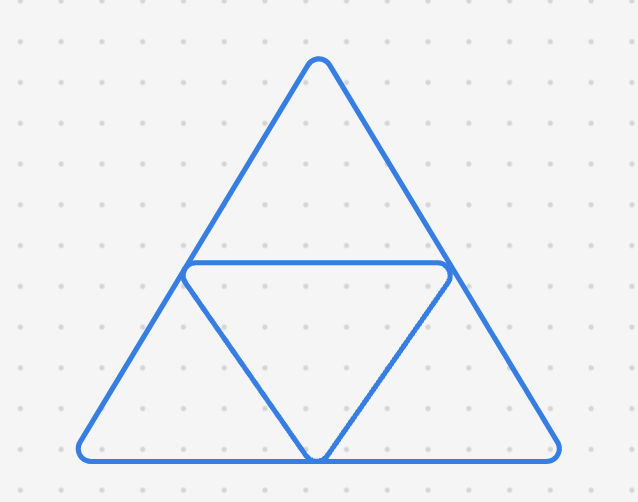
\includegraphics[width=\textwidth]{lection7_1.png}
\end{minipage}
\begin{minipage}{0.65\textwidth}
    \[\text{Разобьём его на 4 $\triangle$ средними линиями и выберем $\Delta_1 :$}\] 
    \[\left|\int_{\partial \Delta_1} f(z) dz\right| \geq \frac{M}{4}\]
    \[\overline{\Delta_0} \supset \overline{\Delta_1} \supset \ldots \supset \overline{\Delta_n} \supset \ldots, \ \left|\int_{\partial \Delta_n} f(z) dz \right| \geq \frac{M}{4^n}\]
\end{minipage}
\[\Rightarrow \exists ! z_0 = \bigcap_{i}^\infty \overline{\Delta_n}, \ z_0 \in D \Rightarrow f \text{ голоморфна в }z_0\]
\[\Rightarrow \forall \epsilon > 0 \ \exists \delta(\epsilon) > 0 : \ \forall z \in U_\delta (z_0) \subset D\]
\[f(z) = f(z_0) + f'(z_0)(z-z_0) + \alpha(z)(z-z_0), \ |\alpha(z)| < \epsilon\]
\[\exists n : \ \Delta_n \subset U_\delta(z)\]
\[\frac{M}{4^n} \leq \left|\int_{\partial \Delta_n} d(z) dz\right| = \left|\int_{\partial \Delta_n} f(z_0) dz + \int_{\partial \Delta_n} f'(z_0)(z-z_0) dz + \int_{\partial \Delta_n} \alpha(z)(z-z_0)dz\right| =\]
\[= \left| \begin{array}{ll}
    \int_\Gamma z^n dz = \frac{\Gamma^{n+1}(b) - \Gamma^{n+1}(a)}{n+1} \\
    n \neq -1
\end{array}\right| = \left|\int_{\partial \Delta_n} \alpha(z)(z-z_0)dz\right| < \epsilon \left| \text{диаметр } \triangle \right| \cdot |\partial \triangle_n|  < \epsilon \cdot |\partial \Delta_n|^2  =\] 
\[= \epsilon \left(\frac{|\partial \Delta_0|}{2^n}\right)^2 = \frac{\epsilon |\partial \Delta_0|^2}{4^n}\]
\[M < \epsilon |\partial \Delta_0|^2 \ \forall \epsilon > 0 \Rightarrow M = 0 \text{ противоречие } \blacktriangleleft\]

\textbfit{Сл.} $\forall$ многоугольника это тоже верно.

\textbfit{Теорема.} Пусть $D \subset \mathbb{C}, D \ -$ область, $f:D \to \mathbb{C}, f \in C(D), \ \gamma \ -$ кусочно-гладкая кривая в $D$. Тогда $\forall \epsilon > 0 \ \exists L \subset D \ - $ ломаная, т.ч. $\left|\int_\gamma f(z) dz - \int_L f(z) dz\right| < \epsilon$.
\[\triangleright \ 1) \ \exists \text { ограниченная область $D_1$, т.ч. } \overline{D_1} \subset D, \ \gamma \subset D_1.\]
\[\forall z \in \gamma \ \exists U_{\delta(z)}(z) \subset D.\] 
\[\text{Рассмотрим } \left\{U_{\frac{\delta(z)}{2}}(z)\right\} \text{ -- покрытие $\gamma$, выберем конечное подпокрытие } \left\{U_{\frac{\delta(z_n)}{2}}(z_n)\right\}_{n=1}^N.\]
\[\text{Положим } D_1 := \bigcup_1^N U_{\frac{\delta(z_n)}{2}}(z_n) \Rightarrow \overline{D_1} \subset D, \gamma \in D_1\]
\[dist (\gamma, \partial D_1) = d > 0\]
\[\text{Тогда будем выбирать разбиение $[a;b]$, по которому пробегает $\gamma$, $z_k = \Gamma(t_k) : |z_{k-1} z_k| < d$.} \]
\[\gamma_k = \Gamma([t_{k-1}, t_k])\]
\[|\gamma_k| = \int_{t_{k-1}}^{t_k} |\dot{\Gamma}(t)| dt \leq M |t_k-t_{k-1}|\]
\[\text{Тогда } L = z_0z_1\ldots z_n \subset D_1\]
\[\overline{D_1} \text{ -- компакт, } \overline{D_1} \subset D \Rightarrow f \in C(\overline{D_1}) \Rightarrow \text{равномерно непрерывная} \Rightarrow\]
\[\Rightarrow \forall \epsilon > 0 \ \exists \delta_1(\epsilon): \ \forall z_1, z_2 : |z_1-z_2| < \delta_1 \Rightarrow |f(z_1)-f(z_2)| < \frac{\epsilon}{|\gamma|}\]
\[\text{Тогда берём разбиение $[a; b]$ т.ч. $|z_{k-1}z_k| < \min(d, \delta_1)$.}\]
\[\left|\int_\Gamma f(z) dz - \int_L f(z) dz\right| = \left|\sum \int_{\Gamma_k}f(z) dz - \sum \int_{[z_{k-1},z_k]}f(z)dz\right| = \left|\sum_{k=1}^n \left(\int_{\Gamma_k}f(z) dz -\right.\right.\] 
\[- \left.\left.\int_{\Gamma_k}f(z_{k-1}) dz \right) + \sum_{k=1}^n \left(\int_{\Gamma_k}f(z_{k-1}) dz - \int_{[z_{k-1},z_k]}f(z) dz\right)\right| =\] 
\[= \left|\int_{\Gamma_k} f(z_{k-1})dz =\int_{[z_{k-1}, z_k]} f(z_{k-1})dz_k \right| \leq \frac{\epsilon}{|\gamma|} \sum_1^n |\Gamma_k| + \sum \left|\int_{[z_{k-1}, z_k]}(f(z_{k-1}) - f(z))dz\right| \leq\]
\[\leq \epsilon + \frac{\epsilon}{|\gamma|} \sum_1^n |z_{k-1}z_k| < \left|\sum_1^n |z_{k-1}z_k| = |L| < |\gamma|\right| < 2\epsilon \ \blacktriangleleft\]

\textbfit{Сл.} (б/д) Пусть $f:\overline{D} \to \mathbb{C}, \partial D \ - $ кусочно-гладкая жорданова замкнутая кривая, $D \ -$ ограниченная область, $f \in C(\overline{D})$. Тогда $\forall \epsilon > 0 \ \exists L \ -$ замкнутая ломаная $L \subset D:$ 

$\left|\int_{\partial D} f(z) dz - \int_L f(z) dz\right| < \epsilon$.

\textit{Отличие от предыдущей теоремы}: в предыдущей теореме наша ломаная может выходить наружу области; эта же теорема говорит, что обязательно сможем построить ломаную, которая полностью лежит внутри области.

\textbfit{Опр.} Область в $\mathbb{C} (\overline{\mathbb{C}})$ называется односвязной, если её граница в $\overline{\mathbb{C}}$ состоит из 0 точек, 1й точки или 1й жордановой кривой (возможно, несобственной).

\subsection{ИТК}
\textbfit{Теорема} (Интегральная теорема Коши для односвязных областей). Пусть $f:D \to \mathbb{C}, f \in \mathcal{O}(D), \overline{G} \subset D, G \ - $ ограниченная односвязная область, $\partial G \ -$ кусочно-гладкая замкнутая жорданова кривая. Тогда $\int_{\partial G} f(z) dz = 0$.
\[\triangleright \text{ По следствию } \forall \epsilon > 0 \ \exists L \subset G \text{ -- замкнутая т.ч. } \left|\int_{\partial G} f dz - \int_L fdz\right| < \epsilon\]
\[\Rightarrow L \text{ -- граница многоугольника } M, \overline{M} \subset G \text{, т.к. $G$ -- односвязная}\]
\[\Rightarrow \text{ по сл. из л. Гурса } \int_L f(z) dz = 0 \Rightarrow \left|\int_{\partial G} f(z) dz\right| < \epsilon \ \forall \epsilon > 0 \Rightarrow \int_{\partial G} f(z) dz = 0 \blacktriangleleft\]

\textbfit{Теорема} (ИТК для многосвязных областей) (б/д). Пусть $f:D\to \mathbb{C}, \overline{G} \subset D, G \ -$ ограниченная область, $\partial G$ состоит из конечного числа замкнутых непересекающихся кусочно-гладких жордановых кривых. Тогда $\int_{\partial G^+} f(z) dz = 0$.

\section{Лекция 8. Первообразная}
\textbfit{Теорема} (Интегральная формула Коши)

Пусть $f \in \mathcal{O} (D),\  G -$ ограниченная область, $\overline{G} \subset D, \ \partial G $
 состоит из конечного числа кусочно-гладких непересекающихся Жордановых кривых, $a \in G$. Тогда $f(a) = \frac{1}{2\pi i} \oint_{\partial G^+} \frac{f(z)}{z-a} dz$

\[\triangleright \ 1) \ a \in G \Rightarrow \exists r > 0: U_r(a) = \{z: |z-a| < r\}, \overline{U_r(a)} \subset G\]
\[\text{Рассмотрим } G_r = G \setminus \overline{U_r(a)}\] 
\[\ \frac{f(z)}{z-a} \in \mathcal{O}(G_r) \overset{\text{ИТК}}{\Rightarrow} \oint_{\partial G_r^+} \frac{f(z)}{z-a} dz = 0 = \oint_{\partial G^+}\frac{f(z)}{z-a}dz + \oint_{(|z-a|=r)^-} \frac{f(z)}{z-a}dz\] 
\[\text{, т.е. } \oint_{\partial G^+} \frac{f(z)}{z-a}dz = \oint_{(|z-a|=r)^+} \frac{f(z)}{z-a}dz\]
\[\text{Л.ч. не зависит от } r\]
\[2) \text{ Хотим } \oint_{(|z-a|=r)^+}\frac{f(z)}{z-a}dz = 2\pi i f(a)\]
\[\int_{|z-a|=r} \frac{1}{z-a}dz = \left|\begin{array}{ll}
z-a=e^{it}r \\
z = \Gamma(t) \\
t \in [0, 2\pi i] \\
\Gamma'(t) = rie^{it}    
\end{array}\right| = \int_0^{2\pi} \frac{1}{r} e^{-it} rie^{it} dt = 2\pi i\]
\[\left|\oint_{(|z-a|=r)^+}\right|\]
\[\ldots \text{см. фото}\]

\textbfit{Теорема} (о среднем)
$f \in \mathcal{O}(D), a \in D, \overline{U_r(a)} \subset D,$ то $f(a) = \frac{1}{2\pi} \int_0^{2\pi} f(a+re^{it})dt$
\[\triangleright \ f(a) \overset{\text{ИФК}}{=} \frac{1}{2\pi i} \oint_{|z-a|=r} \frac{f(z)}{z-a} dz = \left|\begin{array}{ll}
    z = a + re^{it} \\
    z' = rie^{it}    
\end{array}\right| = \frac{1}{2\pi i} \int \frac{f(a+re^{it})}{re^{it}}rie^{it} dt =\] 
\[\frac{1}{2\pi} \int_0^{2\pi} f(a+re^{it})dt \ \blacktriangleleft\]

\textbfit{Пр.}
\[\oint_{\partial \triangle^+} \frac{1}{z} dz = \begin{cases}
    0, \ 0\notin \overline{\triangle} \text{ треугольник с замыканием} \\
    2\pi i f(a) = 2\pi i, \ 0 \in \triangle
\end{cases}\]
\[f(z) = 1, a = 0\in \overline{G} = \overline{\triangle}\]

\subsection{Первообразная}
\textbfit{Опр.} Первообразной $f$ в области $D$ называется $F \in \mathcal{O}(D): F' = f$

\textbfit{Теорема} Пусть $F_1, F_2 -$ первообразные $f$ в области $D$. Тогда $F_1-F_2 \equiv  const$ в $D$.
\[\triangleright \ \text{Рассмотрим } \Phi = F_1 - F_2, \Phi' \equiv 0 \text{ в } D. \ \frac{\partial \Phi}{\partial \overline{z}} \overset{\text{К-Р}}{=} 0, \ \frac{\partial \Phi}{\partial z} = 0 = \Phi'(z) \Rightarrow u_x = u_y = v_x = v_y = 0\]
\[\text{Пусть } \exists a, d, \in D: \Phi(a) \neq \Phi(b) \Rightarrow \exists \Gamma(t) \text{ -- путь в $D$ от $a$ до $b, \ t \in [0, 1]$. } g(t) = \Phi(\Gamma(t)), g' =\] 
\[=\Phi'(\Gamma(t)) \Gamma'(t) = \left(\begin{array}{ll}
    u_x & u_y \\
    v_x & v_y    
\end{array}\right) \left(\begin{array}{ll}
    x'(t) \\
    y'(t)
\end{array}\right) = 0\]
\[\Rightarrow g \equiv const \Rightarrow \Phi(a) = \Phi(b) \text{ -- противоречие } \blacktriangleleft\]

\textbfit{Формула} Ньютона-Лейбница. Пусть $f \in C(D), F -$ первообразная $f$ в $D, \ \Gamma:[a, b] \to D -$ кусочно-гладкий путь. $\int_\Gamma f(z) dz = F(\Gamma(b)) - F(\Gamma(a))$
\[\triangleright \ \int_\Gamma f(z) dz = \int_a^b F'(z) \Gamma'(t) dt = \int_a^b (F(\Gamma(t)))' dt = F(\Gamma(t))\Big|_a^b \ \blacktriangleleft\]

\textbfit{Пр.} $f(z) = \frac{1}{z^2}, \ f \in \mathcal{O} (\mathbb{C} \setminus \{0\})$
\[\exists F = -\frac{1}{z} \in \mathcal{O} (\mathbb{C} \setminus \{0\}) \Rightarrow \int_{\partial \triangle} \frac{1}{z^2} dz = 0\]
\[\nexists \text{ первообразной } f(z) = \frac{1}{z} \text{ в } \mathbb{C} \setminus \{0\} \text{, т.к. } \oint_{|z|=1} \frac{1}{z} dz = 2\pi i\]

\textbfit{Теорема} (о существовании первообразной в круге)

Пусть $F \in C(U_R (a))$ (непрерывна в круге с центром $a$) $\forall \overline{\triangle} \subset U_R(a) \ \int_{\partial \triangle} f(z) dz = 0$. Тогда у $f \ \exists$ первообразная в $U_R(a).$
\[\triangleright \ F(z) = \int_{[a, z]} f(z) dz\]
\[\text{Покажем, что } F'(z) = f(z)\]
\[\frac{F(z+h) - F(z)}{h} - f(z) = \frac{1}{h} \left(\int_{[a, z+h]}f(\zeta) d\zeta - \int_{[a, z]} f(\zeta) d\zeta\right) - f(z) = (*)\]
\[\oint_{\partial \triangle} f(\zeta) d\zeta = \int_{a, z} f(\zeta) d\zeta + \int_{[z, z+h]} - \int_{a, z+h}\]
\[\left(\int_{[a, z+h]}f(\zeta) d\zeta - \int_{[a, z]} f(\zeta) d\zeta\right) = \int_{[z, z+ h]}f(\zeta)d\zeta\]
\[(*) = \frac{1}{h} \int_{[z, z+h]}f(\zeta) d\zeta - f(z) = \frac{1}{h} \int_{[z, z+h]}f(\zeta) d\zeta - \frac{1}{h}\int_{[z, z+h]} f(z) d\zeta = \frac{1}{h} \int_{[z, z+h]}(f(\zeta) - f(z))d\zeta\]
\[\left|\frac{F(z+h) - F(z)}{h} - f(z)\right| \leq \frac{1}{|h|} \sup_{\zeta \in [z, z+h]} |f(\zeta)-f(z)| \cdot |h| \underset{h\to 0}{\to} 0 \ \blacktriangleleft\]

\textbfit{Сл.} $f \in \mathcal{O}(U_R(a)) \Rightarrow \ \exists F -$ первообразная $f$ в $U_R(a).$

\textbfit{Теорема} (критерий существования первообразной в области)

Пусть $f \in C(D).$ Тогда у $f$ в $D \ \exists$ первообразная $\Leftrightarrow \forall$ замкнутого пути $\Gamma:[a, b]\to D \ \oint_\Gamma f(z) dz = 0$
\[\triangleright \ (\Rightarrow) \text{ т. Ньютона-Лейбница}\]
\[(\Leftarrow) \text{ Заметим, что } \int_{\Gamma_1} f(z) dz = \int_{\Gamma_2} f(z) dz\]
\[\Gamma_1, \Gamma_2 - \text{ пути от $a$ до $b$ в $D$. Т.к. путь } \Gamma_1 \cup \Gamma_2^- \text{ замкнут}\]
\[\text{Зафиксируем $a \in D. \ \forall z$ положим } F(z) = \int_{\Gamma_{a, z}} f(z) dz \text{ по любому произвольному $\Gamma$ от $a$}\]
\[\text{до. $z \ (\exists$ т.к. область связна). Покажем, что } F'(z) = f(z). \text{ Т.к. $D$ - область} \Rightarrow\]
\[\Rightarrow \exists r > 0: \overline{U_r(z)} \subset D \Rightarrow \forall h: |h| < r \ z+ h\in D\]
\[\frac{1}{h} (F(z+h) - F(z)) - f(z)\]
\[F(z+h) = \int_{a, z+h}, \ F(z) = \int_{a, z}\]
\[\text{Рассмотрим путь } \Gamma_{a, z+h} = \Gamma_{a, z} \cup [z, z+h] \ F(z+h) - F(z) = \int_{[z, z+h]}f(z) dz\]
\[\text{Длаьше, как в пред теореме } \blacktriangleleft\]

\textbfit{Сл.} Пусть $f \in \mathcal{O}(D), \ D - $ односвязная область. Тогда $\exists F -$ первообразная $f$ в $D$.
\[\triangleright \ \text{Пусть $\Gamma -$замкнутый Жорданов путь в $D$, то $\Gamma$- граница $G: \overline{G} \subset D$}\]
\[\text{По ИТК для односвязных областей } \oint_\Gamma f(z) = 0 \Rightarrow \text{ по критерию $\exists$ первообразная в $D$. } \blacktriangleleft\]


\section{Лекция 9. Формула Тейлора}
Из курса матанализа известно и сразу выполняется:
\[S - \sum_{i=1}^N z_n \underset{N\to \infty}{\to} 0\]
\[f_n(z) \overset{K}{\rightrightarrows } f(z) \overset{def}{\Leftrightarrow} \sup_{z \in K} |f_n(z) - f(z)| \underset{n\to \infty}{\to} 0\]
\[f_n(z) \in C(X) \ f_n \overset{X}{\rightrightarrows } \Rightarrow f \in C(X)\]
\[\sum_{i=1}^\infty f_n(z), \ |f_n(z)| \leq b_n, \ \sum_{i=1}^\infty b_n < \infty \Rightarrow \sum_{i=1}^\infty f_n(z) \rightrightarrows\]
\[f_n(t) \overset{[a, b]}{\rightrightarrows }  f(t), \ \int_a^b f_n(t) dt \to \int_a^b f(t) dt\]
\textbfit{Утв.} Пусть $f_n:\gamma \to \mathbb{C}, \ f_n \in C(\gamma), \ \gamma \ -$ кусочно-гладкая, $f_n \overset{\gamma}{\rightrightarrows} f$. Тогда $\int_\gamma f_n(z) dz \to \int_\gamma f(z) dz$.
\[\triangleright \ \Gamma:[a, b] \to \gamma \text{ -- параметр } \gamma\]
\[\int_\gamma f_n(z) dz = \int_a^b f_n(\Gamma(t)) \dot{\Gamma}(t) dt\]
\[f_n(\Gamma(t))\dot{\Gamma}(t) \rightrightarrows f(\Gamma(t))\dot{\Gamma}(t)\]
\[\underset{t \in [a, b]}{\sup} \left|(f_n(\Gamma(t))-f(\Gamma(t)))\dot{\Gamma}(t)\right| \leq \underset{t \in [a, b]}{\sup} |\dot{\Gamma}(t)|\cdot \underset{t \in [a, b]}{\sup} |f_n(\Gamma(t)) - f(\Gamma(t))| = \underset{t \in [a, b]}{\sup} |\dot{\Gamma}(t)|\times\]
\[\times \underset{z \in \gamma}{\sup} |f_n(z) - f(z)| \to 0\]
\[\int_\gamma f_n(z) dz = \int_a^b f_n(\Gamma(t)) \dot{\Gamma}(t) dt \to \int_a^b f(\Gamma(t))\dot{\Gamma}(t) dt = \int_\gamma f(z) dz \blacktriangleleft\]

\subsection{Формула Тейлора}
\textbfit{Теорема} (Тейлора). Пусть $f \in \mathcal{O}(D), U_R(a) \subset D$. Тогда $c_n = \frac{1}{2\pi i} \oint_{|\zeta - a|=r}\frac{f(\zeta)}{(\zeta-a)^{n+1}}d\zeta, 0<r<R,$
 не зависят от выбора $r$ и называются коэффициентами Тейлора. Ряд $\sum_{n=0}^\infty c_n(z-a)^n$ называется рядом Тейлора $f$ с центром в точке $a, \ \forall z \in U_R(a) \ f(z) = \sum_{n=0}^\infty c_n (z-a)^n$.
\[\triangleright \ 1) \text{ Покажем, что $c_n$ не зависят от $r$. } 0<r_1<r_2<R\]
\[\text{Рассмотрим } G = \{z: r_1 <|z-a|<r_2\}, \ \frac{f(\zeta)}{(\zeta-a)^{n+1}} \in \mathcal{O}(D)\]
\[\overline{G} \subset G_\epsilon = \{z : r_1-\epsilon < |z-a| < r_2 + \epsilon\}, \ \frac{f(\zeta)}{(\zeta-a)^{n+1}}\in \mathcal{O}(D)\]
\[\overset{\text{ИТК}}{\Rightarrow} \oint_{\partial G^+}\frac{f(\zeta)}{(\zeta-a)^{n+1}}d\zeta = 0 = \oint_{(|\zeta-a|=r_2)^+} - \oint_{(|\zeta-a|=r_1)^+}\]
\[2) \text{ фиксируем } z \in U_R(a), \text{ выберем } r: |z-a|<r<R\]
\[\text{По ИФК } f(z) = \frac{1}{2\pi i} \oint_{(|\zeta-a|=r)^+} \frac{f(\zeta)}{\zeta-z}d\zeta = \frac{1}{2\pi i} \oint_{(|\zeta-a|=r)^+} f(\zeta) \frac{1}{\zeta -a - (z-a)} d\zeta =\] 
\[=\left||\zeta-a|>|z-a|\right| = \frac{1}{2\pi i} \oint_{|\zeta-a|=r} \frac{f(\zeta)}{\zeta - a} \cdot \frac{1}{1-\frac{z-a}{\zeta-a}} d\zeta = \frac{1}{2\pi i} \oint_{|\zeta-a|=r} \frac{f(\zeta)}{\zeta-a} \sum_{n=0}^\infty \frac{(z-a)^n}{(\zeta-a)^n}=\]
\[= \frac{1}{2\pi i} \oint_{|\zeta-a|=r} \left( \sum_{n=0}^\infty \frac{f(\zeta)}{(\zeta-a)^{n+1}} (z-a)^n d \zeta \right) = (*)\]
\[\text{Хотим равномерную сходимость } \sum_{n=0}^\infty \frac{f(\zeta)}{(\zeta-a)^{n+1}}(z-a)^n \text{ на } |\zeta-a|=r\]
\[\left|\frac{f(\zeta)}{(\zeta-a)^{n+1}}(z-a)^n\right| \leq |M = \sup f| \leq \frac{M |z-a|^n}{r^{n+1}}\]
\[\frac{M}{r} \sum_{n=0}^\infty \left(\frac{|z-a|}{r}\right)^n < \infty\]
\[(*) = \sum_{n=0}^\infty (z-a)^n \left(\frac{1}{2\pi i} \oint_{|\zeta-a|=r} \frac{f(\zeta)}{(\zeta-a)^{n+1}}d\zeta\right)\]

\textbfit{Сл.} (Неравенство Коши для коэффициентов Тейлора). 
В условиях предыдущей теоремы справедливо неравенство $|c_n| \leq \frac{M_r}{r^n}, \ M_r = \underset{|z-a|=r}{\sup} f(z)$.
\[\triangleright \ |c_n| = \left|\frac{1}{2\pi i} \oint_{|\zeta-a|=r} \frac{f(\zeta)}{(\zeta-a)^{n+1}}d\zeta\right| \leq \frac{1}{2\pi} \cdot \frac{\underset{|\zeta-a|=r}{\sup}|f(\zeta)|}{r^{n+1}} \cdot 2\pi r \ \blacktriangleleft\]

\textbfit{Теорема} (Лиувилля).
Пусть $f \in \mathcal{O}(\mathbb{C}), \exists M > 0 : \forall z \in \mathbb{C} \ |f(z)| \leq M$. Тогда $f \equiv const$.
\[\triangleright \ a = 0, \ f(z) = \sum_{n=0}^\infty c_n z^n \ \forall z \in \mathbb{C}\]
\[\text{По нер-ву Коши } |c_n| \leq \frac{M_r}{r^n} \leq \frac{M}{r^n} \ \forall r > 0\]
\[\frac{M}{r^n} \overset{r\to\infty}{\to}0 \text{ при } n > 0\]
\[\Rightarrow c_n = 0 \ \forall n = 1, 2 \ldots \Rightarrow f(z) = c_0 \ \forall z \in \mathbb{C} \blacktriangleleft\]

\textbfit{Опр.} Функция $f \in \mathcal{O}(\mathbb{C})$ называется целой.

\textbfit{Теорема} (Коши-Адамара).
Пусть есть ряд вида $\sum_{n=0}^\infty b_n (z-a)^n$. Назовём $R = \frac{1}{\overline{\lim_{n\to\infty}} \sqrt[n]{|b_n|}}$ (в т.ч. $\frac{1}{\infty} = 0, \frac{1}{0} = \infty$) радиусом сходимости степенного ряда.
Тогда $\forall z \in U_R(a)$ ряд сходится, $\forall z : |z-a|>R$ ряд расходится. (док-во как в и для вещественных (там смотрим на модули))

\textbfit{Пр.} 
\[\sum_{n=1}^\infty \frac{z^n}{n^2}, \ R = 1, \left|\frac{z}{n^2}\right| = \left|\frac{1}{n^2}\right| \Rightarrow \text{ сходится } \forall z: |z| = 1\]
\[\sum_{n=1}^\infty \frac{z^n}{n}, \ R = 1, \ z = 1 \text{ расходится}, \forall z \neq 1, |z|=1 \text{ сходится}\]
\[\sum_{n=1}^\infty z^n, \ R = 1, \forall z : |z|=1 \text{ расходится}\]

\textbfit{Теорема} (Абеля).
$\sum_{n=0}^\infty b_n(z-a)^n -$ степенной ряд, $R - $ радиус сходимости. $K - $ компакт, $K \subset U_R(a)$. Тогда $\sum_{n=0}^\infty b_n(z-a)^n \overset{K}{\rightrightarrows}$ 
\[\triangleright \ \forall \ 0<r<R \ \sum_{n=0}^\infty |b_n| r^n \text{ сходится}\]
\[\sup_{z \in K} |z-a| = |z_a-a|, z_1 \in K \Rightarrow |z_a-a|=r < R\]
\[\text{Тогда } b_n(z-a)^n \leq |b_n| r^n \ \forall z \in K \Rightarrow \text{ по пр. Вейерштрасса } \sum_{n=0}^\infty b_n(z-a)^n \overset{K}{\rightrightarrows} \ \blacktriangleleft\]

\textbfit{Теорема} (о единственности разложения в ряд Тейлора).
Пусть $f \in \mathcal{O}(U_R(a)), \ \forall z \in U_R(a) \ f(z) = \sum_{n=0}^\infty b_n(z-a)^n.$ Тогда $b_n=c_n.$
\[\triangleright \ c_n = \frac{1}{2\pi i} \oint_{|\zeta-a|=r} \frac{f(\zeta)}{(\zeta-a)^{n+1}}d\zeta = \frac{1}{2\pi i} \oint_{|\zeta-a|=r} \frac{1}{(\zeta-a)^{n+1}} \left(\sum_{k=0}^\infty b_k(\zeta-a)^k\right) d\zeta =\]
\[=\frac{1}{2\pi i} \oint_{|\zeta-a|=r} \left(\sum_{k=0}^\infty b_k(\zeta-a)^{k-n-1}\right) d\zeta = (*)\]
\[R \text{ тот же, } |\zeta-a|=r \text{ компакт. Тогда по т. Абеля }\]
\[(*) = \frac{1}{2\pi i} \sum_{k=0}^\infty b_k \oint_{|\zeta-a|=r} (\zeta-a)^{k-n-1}d\zeta = \begin{cases}
    0, & k-n-1 \neq -1 \\
    2\pi i, & k - n - 1 = -1
\end{cases} = \frac{1}{2\pi i} b_n \cdot 2\pi i = b_n \blacktriangleleft\]
\section{Лекция 10. Бесконечная дифференцируемость голоморфных функций. ИФК для производных. 3 эквивалентных определения голоморфности. Нули}

\textbfit{Теорема} (о голоморфности суммы степенного ряда). Пусть $f(z) = \sum_{n=0}^\infty c_n(z-a)^n, \ R > 0$ -- радиус сходимости. Тогда $f \in \mathcal{O}(U_R(a))$, причём $f'(z) = \sum_{n=1}^\infty c_n \cdot n(z-a)^{n-1}$.
\[\triangleright \ 1) \ g(z) = \sum_{n=1}^\infty c_n \cdot n (z-a)^{n-1}, \text{ тот же радиус сходимости } R\]
\[\text{По т. о $\exists$ первообразной в круге: } \begin{array}{ll}
    1) \ g(z) \in C(U_R(a)) \\
    2) \ \int_{\partial \triangle} g(z) dz = 0
\end{array}\Big| \Rightarrow \exists \text{ первообразная } g(z) \text{ в } U_{R}(a)\]
\[\text{Проверим условия: } 1) \ \forall z_0 \in U_R(a) \ z_0 \in U_r(a): \ r < R, \ \overline{U_r}(a) \subset U_R(a), \text{ ряд сходится } \overset{\overline{U_r}(a)}{\rightrightarrows}\]
\[\Rightarrow g(z) \in C(\overline{U_r}(a)) \Rightarrow g(z) \in C(z_0) \ \forall z \in U_R(a) \Rightarrow g \in C(U_R(a))\]
\[2) \ \int_{\partial \triangle} g(z) dz = \int_{\partial \triangle} \sum_{n=1}^\infty c_n\cdot n (z-a)^{n-1}dz \overset{\text{ряд } \overset{\partial \triangle}{\rightrightarrows}}{=} \sum_{n=1}^\infty \int_{\partial \triangle} c_n \cdot n (z-a)^{n-1} dz = 0\]
\[\Rightarrow \exists \ f_0 \text{ -- первообразная $g$ в } U_R(a)\]
\[f_0(z) = \int_{[a, z]} g(\zeta) d\zeta = \int_{[a, z]} \left(\sum_{n=1}^\infty c_n \cdot n(\zeta-a)^{n-1}\right)d\zeta = \sum_{n=1}^\infty \int_{[a, z]} c_n \cdot n (\zeta - a)^{n-1}d\zeta =\] 
\[=\sum_{n=1}^\infty c_n (\zeta - a)^n \Big|_a^z = \sum_{n=1}^\infty c_n(z-a)^n = f(z) - c_0\]
\[f_0(z) \text{ -- первообразная } \Rightarrow f \in \mathcal{O}(U_R(a))\Rightarrow f(z) = f_0(z) + c_0 \in \mathcal{O}(U_R(a)), \ f'(z) = g(z) \ \blacktriangleleft\]

\subsection{Бесконечная дифференцируемость голоморфных функций}
\textbfit{Теорема} (о бесконечной дифференцируемости голоморфной функции). Пусть $f \in \mathcal{O}(D).$ Тогда $\forall n \in \mathbb{N} \ \exists f^{(n)}$ в $D$, причём $f^{(n)}\in \mathcal{O}(D)$ и $\forall a \in D$ ряд Тейлора для $f^{(n)}$ с центром в т. $a$ получается дифференцированием соответственного ряда для $f$.
\[\triangleright \ f \in \mathcal{O}(U_R(a)) \overset{\text{по т. Тейлора}}{\Rightarrow} f(z) = \sum_{n=0}^\infty c_n(z-a)^n \text{ в } U_R(a) \Rightarrow \text{ по т. о голоморфности суммы }\]
\[\text{степенного ряда } f'(z) = \sum_{n=1}^\infty c_n \cdot n (z-a)^{n-1} \text{ в } U_R(a) \Rightarrow f' \in \mathcal{O}(U_R(a)) \ \blacktriangleleft\]

\textbfit{Следствие} (о виде коэффициентов Тейлора). $c_n = \frac{f^{(n)}(a)}{n!}$
\[\triangleright \ f \in \mathcal{O}(U_R(a)) \Rightarrow f^{(n)} \in \mathcal{O}(U_R(a)) \text{ и }\]
\[\forall z \in U_R(a) \ f^{(n)}(z) = \sum_{k=n}^\infty c_k \cdot k \cdot (k-1) \cdot \ldots \cdot (k-n+1)(z-a)^{k-n}\]
\[\text{Подставим } z=a \ f^{(n)}(a) = c_n \cdot n \cdot (n-1) \cdot \ldots \cdot (n-n+1) = n! \ \blacktriangleleft\]

\subsection{ИФК для производных}
\textbfit{Теорема} (ИФК для производных). Пусть $f \in \mathcal{O}(D), \ G$ -- ограниченная область, $\overline{G} \subset D, \ \partial G$ -- конечное число непересекающихся кусочно-гладких жордановых кривых. Тогда $\forall a \in G \ f^{(n)}(a) = \frac{n!}{2\pi i} \oint_{\partial G^+} \frac{f(z) dz}{(z-a)^{n+1}}$.
\[1) \ \triangleright \ \forall a \in G \ \exists r \geq 0: \ \overline{U_r(a)} \subset G. \ c_n = \frac{1}{2\pi i} \oint_{(\partial U_r(a))^+} \frac{f(z)}{(z-a)^{n+1}}dz = \frac{f^{(n)}(a)}{n!} \Rightarrow \]
\[\Rightarrow f^{(n)}(a) = \frac{n!}{2\pi i} \oint_{(\partial U_r(a))^+} \frac{f(z)}{(z-a)^{n+1}}dz\]
\[2) \ \text{Рассмотрим } G \setminus \overline{U_r}(a). \ \frac{f(z)}{(z-a)^{n+1}} \in \mathcal{O}(G\setminus \overline{U_r}(a)) \overset{\text{ИТК}}{\Rightarrow} \oint_{\partial (G \setminus \overline{U_r}(a))} \frac{f(z)}{(z-a)^{n+1}}dz = 0 =\]
\[= \oint_{\partial G^+} - \int_{(\partial U_r(a))^+} \Rightarrow f^{(n)}(a) = \frac{n!}{2\pi i} \oint_{\partial G^+} \frac{f(z)}{(z-a)^{n+1}} dz \blacktriangleleft\]

\textbfit{Теорема} (о восстановлении голоморфной функции по вещественной части)

1) Пусть $f \in \mathcal{O}(D), \ u = \re f$. Тогда $u$ -- гармоническая в $D$, т.е. $u \in C^2(D)$ и $\Delta u = u_{xx}+u_{yy} = 0$ в $D$.

2) Пусть $u$ -- гармоническая в $D$, $D$ -- односвязная область. Тогда $\exists !$ с точностью до мнимой константы $f \in \mathcal{O}(D): \ \re f = u$.
\[\triangleright \ 1) \ f \in C^2(D) \Rightarrow u = \re f \in C^2(D) \overset{\text{К-Р}}{\Rightarrow} \Delta u = 0\]
\[(u_{xx} + u_{yy} = (v_y)'_x + (-v_x)'_y = v_{yx} - v_{xy}=0, \text{ по т.Шварца, т.к. } v = \im f \in C^2(D))\]
\[2) \ \text{Хотим } f = u + iv \Rightarrow f' = u_x + iv_x = u_x-iu_y\]
\[\text{Рассмотрим } g = u_x -iu_y \ (f' \text{обязана иметь такой вид})\]
\[g \ \mathbb{R}\text{-дифференцируема, т.к. } u \in C^2(D), \text{ и выполнено К-Р, т.к. } (u_x)_x = (-u_y)_y \text{ -- верно, т.к. } \]
\[u_{xx}+u_{yy} = 0 \text{ в } D, \ (u_x)_y=-(-u_y)_x \text{ -- верно по т. Шварца, т.к. } u \in C^2(D) \Rightarrow g \in \mathcal{O}(D)\]
\[\text{Т.к. $D$ -- односвязная, то у } g \ \exists \text{ первообразная } f_0\]
\[f_0(z) = U + iV, \ \text{ но т.к. } f_0' = g, \text{ то } U'_x = u_x, \ U'_y = u_y \text{ в } D \Rightarrow U - u \equiv const\]
\[\text{Выберем } c = 0. \text{ Тогда } \re f_0 = u, \ f_0 \in \mathcal{O}(D).\]
\[V'_x = -u_y, \ V'_y = u_x \Rightarrow V \text{ определяется с точностью до константы.} \ \blacktriangleleft\]

\textbfit{Теорема} (Мореры). Пусть функция $f$ удовлетворяет условию трегольника: $f \in C(D), \ \forall \overline{\triangle} \subset D, \ \oint_{\partial \triangle} f(z) dz = 0.$ Тогда $f \in \mathcal{O}(D).$
\[\triangleright \ \forall a \in D \ \exists R>0: \ U_R(a) \subset D.\] 
\[\text{Тогда для $f$ в } U_R(a) \text{ выполнено условие $\exists$ первообразной в круге.} \Rightarrow\] 
\[\Rightarrow \exists F \in \mathcal{O}(U_R(a)) : F' = f \Rightarrow f \in \mathcal{O}(U_R(a)) \text{ по т. о бесконечной дифференцируемости} \Rightarrow\]
\[\Rightarrow  f \in \mathcal{O}(D) \blacktriangleleft\]
\subsection{3 эквивалентных определения голоморфности}
\textbfit{Теорема} (3 эквивалентных определения голоморфности). Следующие утверждения эквивалентны:

1) $\forall a \in D \ \exists R > 0 :$ в $U_R(a)$ выполнено условие Коши-Римана.

2) $f$ аналитична в $D$, т.е. $\forall a \in D \ \exists R > 0: \ f(z) = \sum_{n=0}^\infty c_n(z-a)^n \ \forall z \in U_R(a)$.

3) условие треугольника: $f \in C(D), \ \forall \overline{\triangle} \subset D \ \oint_{\partial \triangle} f(z) dz = 0.$
\[\triangleright \ (1) \overset{\text{л. Гурса}}{\Rightarrow} (3), \ (3) \overset{\text{т. Мореры}}{\Rightarrow} (1)\]
\[(1) \overset{\text{т. Тейлора}}{\Rightarrow} (2), \ (2) \overset{\text{т. о голоморфности суммы степенного ряда}}{\Rightarrow} (1) \ \blacktriangleleft\]

\subsection{Нули}
\textbfit{Теорема} (о поведении функции в окрестности нуля). Пусть $f \in \mathcal{O}(D), \ a \in D, \ f(a) = 0. \ \exists R>0, \exists n \in \mathbb{N} : \ f(z) = (z-a)^n g(z),$ где $g \in \mathcal{O}(U_R(a)), \ g(z) \neq 0$ в $U_R(a)$ (или $\exists R> 0: \ f \equiv 0$ в $U_R(a)$).
\[\triangleright \ \text{в } U(a) \ f(z) = \sum_{n=0}^\infty c_n (z-a)^n, \ c_0 = f(a) = 0\]
\[\text{Если } \forall n \ c_n =0, \text{ то } f(z) \equiv 0 \text{ в } U(a).\] 
\[\text{Иначе положим } N := \inf \{n: c_n \neq 0\}.\] 
\[\text{Тогда } g(z) := \sum_{n = N}^\infty c_n (z-a)^{n-N} \text{ сходится в том же круге.}\]
\[g(a) = c_N \neq 0, \ g \in \mathcal{O}(U(a)) \Rightarrow \exists R>0: g(z) \neq 0 \text{ в } U_R(a), \ f(z) = (z-a)^N g(z) \text{ в } U_R(a) \blacktriangleleft\]

\textbfit{Опр.} Пусть $f \in \mathcal{O}(D), \ a \in D, \ f(a) = 0$. Тогда $N = \inf \{n:c_n \neq 0\} = \inf \{n: f^{(n)}(a) \neq 0\}$ называется порядком нуля $f(z)$ в т. $a$.

\textbfit{Утв.} (об изолированности нулей голоморфной функции). Пусть $f \in \mathcal{O}(D), \ f(a) = 0$. Тогда либо $\exists R > 0: f(z) \equiv 0$ в $U_R(a)$, либо $\exists R>0: f(z) \neq 0$ в $\mathring{U_R}(a)$.
\[\triangleright \text{ Очев. (из пред. факта)} \blacktriangleleft\]

\textbfit{Пр.} $f(z) = \frac{\sin^2 z \cos z}{z}, \ f(0) := 0, \ f \in \mathcal{O}(D).$
\[\sin z \text{ -- порядок 1} \Rightarrow \sin z = (z-0) g(z), \ g(z) \neq 0\]
\[f(z) = \frac{z^2 g^2(z) \cos z}{z} = zg^2(z) \cos z, \ g^2(z) \cos z \neq 0 \text{ в некоторой окрестности 0} \Rightarrow \text{порядок 1}\]
\section{Лекция 11. Теорема о единственности. Теорема Вейерштрасса}
\textbfit{Опр.} Пусть $f(\infty) = 0, \ f\in \mathcal{O}(|z|>R)$. Тогда порядком нуля в бесконечности называют порядок нуля $f\left(\frac{1}{z}\right)$ в 0.

$g(z) = f\left(\frac{1}{z}\right) = z^N \tilde{g}(z), \ \tilde{g}(z) \neq 0$

$f(z) = g \left(\frac{1}{z}\right) = \frac{\tilde{g}\left(\frac{1}{z}\right)}{z^N} = \frac{1}{z^N}g_1(z), \ \tilde{g} \left(\frac{1}{z}\right) \neq 0$

\subsection{Теорема о единственности}
\textbfit{Теорема} (о единственности). Пусть $f, g \in \mathcal{O}(D), f \overset{E}{=} g, \ E \subset D, E $ имеет предельную точку в $D.$ Тогда $f \overset{D}{=} g.$
\[\triangleright \text{ Рассмотрим } F = f - g, \ F \in \mathcal{O}(D), F \overset{E}{=} 0\]
\[\text{Пусть $a$ -- предельная точка } E, a \in D \Rightarrow F(a) = 0 \text{. Тогда $a$ -- неизолированный ноль.} \Rightarrow\]
\[\Rightarrow \exists U_R(a) \subset D: F = 0 \text{ на } U_R(a)\]
\[\text{Пусть } \exists b \in D: F(b) \neq 0 \text{. Рассмотрим путь } \Gamma:[0, 1] \to D: \Gamma(0) = a, \Gamma(1) = b\]
\[\text{Пусть } T = \inf \{t \in [0, 1]: F(\Gamma(t)) \neq 0\} \text{ -- непусто, ограничено}\]
\[T > 0, \text{ т.к. } \exists \delta: \forall t < \delta \Gamma(t) \in U_R(a) \Rightarrow F(\Gamma(t))=0\]
\[T \neq 1 \text{ в силу непрерывности } F \text{ (иначе $F(b) = 0$)}\]
\[0 < T < 1. \text{ По непрерывности } F(\Gamma(T)) = 0 \Rightarrow \Gamma(T) \text{ -- неизолированный ноль} \Rightarrow\]
\[\Rightarrow \exists U_r(\Gamma(T)): \forall z \in U_r(\Gamma(T)) \ F(z) = 0 \Rightarrow \exists \delta_1: \forall t \in (T, T + \delta_1) \ \Gamma(t) \in U_r(\Gamma(T)), F(\Gamma(t)) = 0 \Rightarrow\]
\[\Rightarrow \nexists \inf \text{ -- противоречие }\blacktriangleleft\]

\textbfit{Пр.} $f \in \mathcal{O}(|z|<1), z_n \to \frac{1}{n} \in U_1(0), f\left(\frac{1}{n}\right) = 0 \Rightarrow f \equiv 0$
\[f \in \mathcal{O}(|z-1|<1), z_n \to \frac{1}{n} \in U_1(0), f \left(\frac{1}{n}\right) = 0 \overset{?}{\Rightarrow} f = \sin \frac{\pi}{z}\]
\[f \in \mathcal{O}(\mathbb{C}), z_n \to n \in U_1(0), f(n) = 0 \overset{?}{\Rightarrow} f = \sin \pi z\]

\textbfit{Замечание} Теоремы Лагранжа не существует в комплексном анализе.

\subsection{Теорема Вейерштрасса}
\textbfit{Теорема} (Вейерштрасса). Пусть $f_n \in \mathcal{O}(D)$. Пусть $\forall K \subset D, K$ -- компакт $f_n \overset{K}{\rightrightarrows} f$ (меньше, чем сходимость на всей $D$). Тогда

1) $f \in \mathcal{O}(D)$

2) $\forall z \in D \ \forall k f_n^{(k)}(z) \to f^{(k)}(z)$

3) $\forall K \subset D, K -$ компакт $f_n^{(k)}(z) \overset{K}{\rightrightarrows} f(z)$
\[\triangleright \ 1) \text{ Покажем } f \in \mathcal{O}(D)\]
\[f \in C(D) \text{ (т.к. $C(D) \ni f_n \overset{K}{\rightrightarrows} f \Rightarrow f \in C(K) \forall z_0 \in D \exists \overline{U_R(z_0)} \subset{D} \Rightarrow f \in C(\overline{U_R(z_0)}) \Rightarrow$}\]
\[\Rightarrow f \in C(z_0) \Rightarrow f \in C(D))\]
\[\text{Пусть } \overline{\triangle} \subset D \int_{\partial \overline{\triangle}} f(z) dz = \int_{\partial \overline{\triangle}} (\lim_{n\to\infty} f_n(z))dz \overset{f_n \overset{\partial \triangle}{\rightrightarrows} f}{=} \lim_{n\to\infty} f_n(z) dz = 0, \ f_n(z) = 0\text{ (л. Гурса)} \Rightarrow\]
\[f \in \mathcal{O}(D) \text{ по т. Мореры}\]
\[2) \text{ Пусть $a \in \triangle$. Покажем } \forall k \lim_{n\to\infty} f_n^{(k)}(a) = f^{(k)}(a)\]
\[\exists R > 0: \overline{U_R(a)} \subset D\]
\[\text{Тогда }f^{(k)}(a) \overset{\text{ИФК}}{=} \frac{k!}{2\pi i} \oint_{|z-a|=R} \frac{f(z)}{(z-a)^{k+1}}dz = \frac{k!}{2\pi i} \oint_{|z-a|=R} \left(\lim_{n\to\infty}\frac{f(z)}{(z-a)^{k+1}}\right)dz = (*)\]
\[\sup_{|z-a|=R} \left|\frac{f_n(z)}{(z-a)^{k+1}} - \frac{f(z)}{(z-a)^{k+1}}\right| = \frac{1}{R^{k+1}}\sup_{|z-a|=R} |f_n(z)-f(z)|<\epsilon \forall n > N \text{ т.к. } f_n \overset{|z-a|=R}{\rightrightarrows} f\]
\[(*) \overset{\text{в силу равномерной сходимости}}{=} \lim_{n\to\infty} \frac{k!}{2\pi i} \oint_{|z-a|=R} \frac{f_n(z)}{(z-a)^{k+1}}dz \overset{\text{ИФК}}{=} \lim_{n\to\infty} f_n^{(k)}(a)\]
\[3) \text{ Сначала покажем, что } \forall a \in D \exists R(a): f_n^{(k)} \overset{\overline{U_{R(a)}(a)}}{\rightrightarrows} f^{(k)}(z)\]
\[\exists r(a) : \overline{U_{r(a)}(a)} \subset D. \text{ Возьмём } 0 < R(a) < r(a).\] 
\[\text{ Тогда } \forall z \in \overline{U_{R(a)}} \ f_n^{(k)}(z) - f^{(k)}(z) = \frac{k!}{2\pi i} \oint_{|\zeta-a|=r(a)} \frac{f_n(\zeta)-f(\zeta)}{(\zeta-z)^{k+1}}d\zeta\]
\[\sup_{|\zeta-a|=r(a)} \left|\frac{k!}{2\pi i}\oint_{|\zeta-a|=r(a)}\frac{f_n(\zeta)-f(\zeta)}{(\zeta - z)^{k+1}} d\zeta\right| \leq \frac{k!}{2\pi i} \cdot \frac{\epsilon}{(r-R)^{k+1}} \text{ т.е. } \rightrightarrows\]
\[\forall K \subset D, K \text{ -- компакт. Рассмотрим } \{U_{R(a)}(a)\}_{a \in K} \text{ -- открытое покрытие, выберем конечное}\]
\[\text{подпокрытие } K \subset \bigcup_{n=1}^N \overline{U_{R_n(a_n)}(a_n)} \text{, т.к. их конечно, то } f_n^{(k)} \overset{\overline{U_{R_n(a_n)}(a_n)}}{\rightrightarrows} f^{(k)} \blacktriangleleft\]

\textbfit{Теорема} (Рунге). Пусть $D -$ односвязная область. $f \in \mathcal{O}(D)$. Тогда $\exists P_n -$ последовательность многочленов: $\forall F \subset D, K -$ компакт $P_n \overset{K}{\rightrightarrows} f$.

\textbfit{Пр.} $f(z) = \frac{1}{z}, \ \mathbb{C} \setminus \{0\}$
\[\oint_{|z|=1} P_n(z) dz = 0 \to \oint_{|z|=1} \frac{1}{z} dz = 2\pi i \Rightarrow \nexists P_n\]

\section{Лекция 12. Ряды Лорана}
\subsection{Ряды Лорана}
\textbfit{Теорема} (Лорана). Пусть $f \in \mathcal{O}(V), \ V = \{z: r < |z-a|< R\}, \ 0 \leq r < R \leq \infty.$ Тогда $\forall z \in V \ f(z) = \sum_{n=-\infty}^{+\infty} c_n (z-a)^n, \ c_n := \frac{1}{2\pi i} \oint_{|z-a|=\rho} \frac{f(z)}{(z-a)^{n+1}}dz, \ r<\rho<R$, где под сходимостью ряда подразумевается, что сходятся оба ряда  $\sum_{n=0}^\infty c_n(z-a)^n, \ \sum_{n=1}^{\infty}c_{-n} (z-a)^{-n}$.
 
$\sum_{n=0}^\infty c_n(z-a)^n$ -- правильная часть ряда Лорана, $\sum_{n=1}^{\infty}c_{-n} (z-a)^{-n}$ -- главная часть ряда Лорана.
\[\triangleright \ 1) \text{ Почему $c_n$ не зависят от $\rho$?}\]
\[\frac{f(z)}{(z-a)^{n+1}} \in \mathcal{O}(\rho_1 < |z-a|<\rho_2), r<\rho_1<\rho_2<R \Rightarrow \oint_{\partial(\rho_1<|z-a|<\rho_2)} \frac{f(z)}{(z-a)^{n+1}}dz = 0 =\]
\[=\left(\oint_{(|z-a|>\rho_2)^+} - \oint_{(|z-a|<\rho_1)^-}\right)\frac{f(z)}{(z-a)^{n+1}}dz\]
\[2) \ \text{Фиксируем } z \in V. \text{ Выберем } r<\rho_1< |z-a|<\rho_2<R\]
\[f(z) \overset{\text{ИФК}}{=} \frac{1}{2\pi i}\oint_{(|\zeta-a|=\rho_2)^+} \frac{f(\zeta)}{\zeta-z}d\zeta - \frac{1}{2\pi i} \oint_{(|\zeta-a|=\rho_1)^+} \frac{f(\zeta)}{\zeta-z}d\zeta = \left|\frac{f(\zeta)}{\zeta-z} =\frac{f(\zeta)}{\zeta-a-(z-a)}\right|=\]
\[=\frac{1}{2\pi i} \oint_{|\zeta-a|=\rho_2} \frac{f(\zeta)}{\zeta -a}\cdot \frac{d\zeta}{1-\frac{z-a}{\zeta-a}} + \frac{1}{2\pi i} \oint_{|\zeta-a|=\rho_1} \frac{f(\zeta)}{z-a} \cdot \frac{d\zeta}{1-\frac{\zeta - a}{z-a}} =\] 
\[=\frac{1}{2\pi i} \oint_{|\zeta-a|=\rho_2}\left(\frac{f(\zeta)}{\zeta-a}\sum_{n=0}^\infty \left(\frac{z-a}{\zeta-a}\right)^n \right)d\zeta +\frac{1}{2\pi i}\oint_{|\zeta-a|=\rho_1}\left( \frac{f(\zeta)}{z-a} \sum_{n=0}^\infty \left(\frac{\zeta-a}{z-a}\right)^n \right)d\zeta =\]
\[=\frac{1}{2\pi i} \oint_{|\zeta-a|=\rho_2} \left(\sum_{n=0}^\infty \frac{f(\zeta)(z-a)^n}{(\zeta-a)^{n+1}}\right)d\zeta+\frac{1}{2\pi i}\oint_{|\zeta-a|=\rho_1} \left(\sum_{n=0}^\infty \frac{f(\zeta)(\zeta-a)^n}{(z-a)^{n+1}}\right)d\zeta = (*)\]
\[|\zeta-a|=\rho_2:\left|\frac{f(\zeta )(z -a)^n}{(\zeta-a)^{n+1}}\right| \leq \frac{M |z-a|^n}{\rho_2^{n+1}}, \ M = \sup_{|\zeta-a|=\rho_2}f\]
\[\frac{M}{\rho_2}\sum_{n=0}^\infty \left(\frac{|z-a|}{\rho_2}\right)^n, \ \frac{|z-a|}{\rho_2} < 1 \Rightarrow \text{сходится} \Rightarrow \text{по признаку Вейерштрасса } \rightrightarrows\]
\[|\zeta-a|=\rho_1:\left|\frac{f(\zeta )(\zeta -a)^n}{(z-a)^{n+1}}\right| \leq \frac{\widetilde{M} \rho_1^n}{|z-a|^{n+1}}, \ \widetilde{M} = \sup_{|\zeta-a|=\rho_1}f\]
\[\frac{\widetilde{M}}{|z-a|}\sum_{n=0}^\infty \left(\frac{\rho_1}{|z-a|}\right)^n, \ \frac{\rho_1}{|z-a|} < 1 \Rightarrow \text{сходится} \Rightarrow \text{по признаку Вейерштрасса } \rightrightarrows\]
\[(*) = \sum_{n=0}^\infty \left(\frac{1}{2\pi i} \oint_{|\zeta-a|=\rho_2} \frac{f(\zeta)}{(\zeta-a)^{n+1}} d\zeta \right) (z-a)^n + \sum_{n=0}^\infty \left(\frac{1}{2\pi i}\oint_{|\zeta-a|=\rho_1}\frac{f(\zeta)}{(\zeta-a)^{-n}} d\zeta\right) \times\]
\[\times (z-a)^{-n-1}\]
\[c_n = \frac{1}{2\pi i} \oint_{|\zeta-a|=\rho_2} \frac{f(\zeta)}{(\zeta-a)^{n+1}} d\zeta, \ c_{-n-1} = \frac{1}{2\pi i}\oint_{|\zeta-a|=\rho_1}\frac{f(\zeta)}{(\zeta-a)^{-n}} d\zeta \ \blacktriangleleft\]

\textbfit{Теорема} (о сходимости ряда Лорана). $\sum_{n=-\infty}^{+\infty} b_n (z-a)^n.$

$R := \frac{1}{\overline{\lim}_{n\to\infty} \sqrt[n]{|b_n|}}$, $r:= \overline{\lim}_{n\to\infty} \sqrt[n]{|b_{-n}|}.$ Тогда ряд сходится, причём абсолютно в $V = \{r < |z-a| < R\}$, и правильная часть расходится при $|z-a|>R$, а главная часть -- при $|z-a| < r$.
При этом $\forall K \subset V, \ K$ -- компакт, ряд сходится равномерно, а $f(z) = \sum_{n=-\infty}^{+\infty} b_n (z-a)^n \ f \in \mathcal{O}(V)$ и $b_n = c_n$.
\[\triangleright \ 1) \ f_1(z) = \sum_{n=0}^\infty b_n (z-a)^n \text{ сходится абсолютно при } |z-a| < R, \text{ расходится при } |z-a| > R.\]
\[f_1 \in \mathcal{O}(|z-a|< R), \ \sum_{n=0}^\infty b_n (z-a)^n \overset{K}{\rightrightarrows} \text{ по т. Абеля.}\]
\[f_2(z) = \sum_{n=1}^\infty \frac{b_{-n}}{(z-a)^n} \text{ сходится абсолютно при } \left|\frac{1}{z-a}\right| < \frac{1}{r} \Leftrightarrow |z-a| > r, \ \text{ расходится при}\]
\[|z-a| < r\]
\[g(w) = \sum_{1}^\infty b_{-n}w^n \ \forall K \in \{|w| < r\} \overset{K}{\rightrightarrows}\]
\[K \overset{\frac{1}{w}}{\to} K_1 \text{ -- компакт}, \ \{0\} \notin K, \frac{1}{w} \in C\]
\[\sup_{w \in K} \left|g(w)-\sum_{n=1}^N b_{-n} w^n\right| = \sup_{z \in K_1} \left|f_2(z) - \sum_{n=1}^\infty b_{-n} (z-a)^{-n}\right| \Rightarrow \sum_{n=1}^\infty b_{-n} (z-a)^{-n} \overset{K}{\rightrightarrows} f_2(z)\]
\[g \in \mathcal{O}(|w|<\frac{1}{r}), \ f_2 = g\left(\frac{1}{z-a}\right) \in \mathcal{O}(|z-a|>r), \text{ т.к. } |z-a|\neq 0 \Rightarrow \frac{1}{z-a} \in \mathcal{O}(|z-a|>r)\]
\[2) \ \text{Покажем } !\]
\[f \in \mathcal{O}(V) \Rightarrow c_n = \frac{1}{2\pi i} \oint_{|\zeta-a|=\rho} \frac{f(\zeta)}{(\zeta-a)^{n+1}}d\zeta = \frac{1}{2\pi i} \oint_{|\zeta-a|=\rho} \frac{1}{(\zeta-a)^{n+1}} \left(\sum_{k=-\infty}^{+\infty} b_k (\zeta-a)^k\right)d\zeta =\] 
\[=\frac{1}{2\pi i} \oint_{|\zeta-a|=\rho} \left(\sum_{k=-\infty}^{+\infty} b_k (\zeta-a)^{k-n-1}\right)d\zeta = (*)\]
\[\sum_{k=-\infty}^{+\infty} b_k (\zeta-a)^{k-n-1} \text{ ряд сдвинут на константу членов } \Rightarrow R, r \text{ не изменились } \Rightarrow \overset{V}{\rightrightarrows}\]
\[(*) = \sum_{k=-\infty}^{+\infty} \frac{b_k}{2\pi i} \oint_{|\zeta-a|=\rho} (\zeta-a)^{k-n-1} d\zeta = \left|\oint_{|\zeta-a|=\rho} (\zeta-a)^{k-n-1} d\zeta = \begin{cases}
    0, \ k-n-1\neq -1 \\
    2\pi i, k = n
\end{cases}\right| =\]
\[ = b_n \ \blacktriangleleft\]

\textbfit{Утв.} Неравенство Коши (для коэффициентов Лорана). 

$|c_n| \leq \frac{M(\rho)}{\rho^n},$ где $M(\rho) = \sup_{|z-a|=\rho} |f(z)|.$
\[\triangleright \text{ Аналогично. } \blacktriangleleft\]

\textbfit{Опр.} Точка $a \in \mathbb{C}$ называется изолированной особой точкой однозначного характера (ИОТОХ), если $f \in \mathcal{O}(0 < |z-a| < \epsilon)$ с некоторым $\epsilon > 0$. При этом 

1) если $\exists \lim_{z\to a} f(z) \in \mathbb{C}$, то $a$ -- устранимая ОТ (УОТ)

2) если $\exists \lim_{z\to a} f(z) = \infty$, то $a$ -- полюс

3) если $\nexists \lim_{z\to a} f(z)$, то $a$ -- существенная ОТ (СОТ).

\textbfit{Теорема} (об описании УОТ). Пусть $a$ -- ИОТ $f$. Тогда следующие утверждения эквивалентны:

1) $a$ -- УОТ

2) $f$ -- ограниченная в некоторой $\mathring{U_{\epsilon'}}(a)$

3) $c_n = 0$ при $n \leq -1$

4) $f$ можно доопределить в т. $a$ до голоморфности
\[\triangleright \ (1) \Rightarrow (2): \text{ если функция имеет предел в т. $a$, то она локально ограничена в этой точке}\]
\[(2) \Rightarrow (3): \ f \text{ ограничена в } \mathring{U_{\epsilon'}}(a)\]
\[\text{При } 0 < \rho < \epsilon' \ M(\rho) \leq M \Rightarrow |c_{-n}| \leq \frac{M(\rho)}{\rho^{-n}} = M(\rho)\rho^n \underset{\rho\to 0}{\to} 0 \Rightarrow c_{-n} = 0 \text{ при } n \geq 1\]
\[(3) \Rightarrow (4): \ \mathring{U_{\epsilon'}}(a) \ f(z) = \sum_{n=0}^\infty c_n (z-a)^n = (*)\]
\[f(a) := c_0 \Rightarrow (*) \text{ выполнено в } U_{\epsilon'}(a) \Rightarrow f \in \mathcal{O}(U_{\epsilon'}(a))\]
\[(4) \Rightarrow (1): \ \text{ очев } \blacktriangleleft\]

\textbfit{Замечание.} Радиус сходимости ряда Лорана (Тейлора) равен расстоянию от центра $a$ до ближайшей ОТ (НО не УОТ, т.к. в ней можем доопределить).
\section{Лекция 13. Связь ряда Лорана с типом ИОТ. Целые и мероморфные функции}
\textbfit{Теорема} Пусть $f \in \mathring{U}_{\epsilon}(a), a -$ полюс $\Leftrightarrow f(z) = \sum_{-N}^{+\infty} c_n(z-a)^n, N >0$
\[\triangleright (\Rightarrow) \lim_{z\to a} f(z) = \infty. \ \frac{1}{f(z)} \in \mathcal{O}(\mathring{U}_{\epsilon'}(a)), \ \lim_{z\to a} \frac{1}{f(z)} = 0 \Rightarrow a - \text{Уот для $\frac{1}{f}$, доопределим в $a$}\]
\[\text{и получим } \frac{1}{f} \in \mathcal{O}(U_{\epsilon'}(a))\]
\[\frac{1}{f} = (z-a)^N h(z), h(z) \neq 0 \text{ в } U_{\epsilon^{''}}(a)\]
\[f(z) = \frac{1}{(z-a)^N} \cdot \frac{1}{h}(z) = \frac{1}{(z-a)^N} \sum_{n=0}^\infty b_n (z-a)^n = \left|b_0 \neq 0\right| = \sum_{n=0}^\infty b_n (z-a)^{n-N} =\]
\[=\sum_{n=-N}^\infty b_{n+N} (z-a)^n\]
\[(\Leftarrow) f(z) = \sum_{n=-N}^\infty c_n (z-a)^n = (z-a)^N \sum_{n=-N}^\infty c_n (z-a)^{n+N} = (z-a)^{-N}\sum_{n=0}^\infty c_{n-N}(z-a)^n\]
\[\sum_{n=0}^\infty c_{n-N}(z-a)^n \in \mathcal{O}(\mathring{U}(a)) \overset{\text{УОТ}}{\Rightarrow} \mathcal{O}(U(a)), (z-a)^{-N} \to \infty \Rightarrow f(z) \to \infty \blacktriangleleft\]

\textbfit{Опр.} Пусть $a -$ плюс $f(z)$. Тогда порядком полюса в т. $a$ называется порядком нуля функции $\frac{1}{f}$ в т. $a$.

\textbfit{Замечание.} $f(z) = \frac{g(z)}{(z-a)^N} \Leftrightarrow a - $ порядок $N, \ g(z) \neq 0 $ в $\mathring{U}(a)$.

\textbfit{Следствие.} $a -$ СОТ $f \Leftrightarrow$ в главное части ряда Лорана $f$ в $\mathring{U}_\epsilon(a)$ бесконечно много ненулевых слагаемых.

\textbfit{Теорема} (Соходского). Пусть $a -$ СОТ функции $f(z)$. Тогда $\forall A \in \overline{\mathbb{C}} \ \exists z_n \to a: f(z_n) \to A.$
\[\triangleright 1) A = \infty. \text{ Пусть $f$ ограничена в некоторой $\mathring{U}(a)$. Тогда $a - $ УОТ} \Rightarrow f \text{ неогр.} \Rightarrow\]
\[\Rightarrow \exists z_n \to a : f(z_n) \to \infty\]
\[2) A \in \mathbb{C}. \text{ Если } \exists z_n \to a: f(z_n) = A, \text{ то победа}\]
\[\text{Иначе построим } g(z) = \frac{1}{f(z)-A} \in \mathcal{O}(\mathring{U}_{\epsilon'}(a))\]
\[f(z) = \frac{1}{g(z)} + A.\] 
\[\text{ Если $a - $ УОТ для $g$, тогда для $f$ это УОТ или полюс - противоречие. Если $a -$ полюс}\]
\[\text{для $g$, то для $f -$ УОТ} \Rightarrow \text{$a -$ СОТ для $g$} \Rightarrow \exists z_n \to a: g(z_n) \to \infty \Rightarrow f(z_n) \to A \blacktriangleleft\]

\textbfit{Опр.} $\infty$ называется ИОТ для $f(z)$, если $\exists R > 0: f \in \mathcal{O}(|z|> R)$. Классификация та же или же тип особой точки в $\infty -$ это тип особой точки в 0 у $f\left(\frac{1}{z}\right)$.

\subsection{Связь типа ИОТ в $\infty$ с рядом Лорана в $|z| > R$}

1) $\infty -$ УОТ $f(z) = \sum_{n=-\infty}^0 c_n z^n$

2) $\infty -$ полюс. $f(z) = \sum_{n=-\infty}^N c_n z^n, N > 0, N -$ порядок полюса, $f(z) = z^N g(z), \ g(z) \neq 0 \in \mathcal{O}(|z|>R)$

3) $\infty -$ СОТ. В разложении бесконечно много слагаемых с положительными степенями.

\textbfit{Теорема.} Если $f \in \mathcal{O}(\mathbb{C}), \ \infty -$ УОТ, то $f \equiv const$
\[\triangleright \text{Т.к. $\infty -$ УОТ, то } \exists R > 0: f(z) \text{ ограничена в } \{|z|>R\}, \text{ а при $|z| \leq R \ f$ ограничена по}\]
\[\text{т. Вейерштрасса} \Rightarrow f \in \mathcal{O}(\mathbb{C}), f \in B(\mathbb{C}) \overset{\text{т. Лиувилля}}{\Rightarrow} f \equiv const \blacktriangleleft\]

\textbfit{Теорема.} Если $f \in \mathcal{O}(\mathbb{C}), \ \infty -$ полюс, то $f -$ многочлен
\[\triangleright f \in \mathcal{O}(\mathbb{C}) \Rightarrow f(z) = \sum_{n=0}^\infty c_n z^n \forall z \in \mathbb{C}\]
\[\text{По т. о связи с рядом Лорана } f(z) = \sum_{n=-\infty}^N c_n z^n \Rightarrow f(z) = \sum_{n=0}^N c_n z^n \blacktriangleleft\]

\textbfit{Опр.} $f \in \mathcal{O}(\mathbb{C}), \ \infty -$ СОТ называются трансцендентными.

\textbfit{Теорема} (малая т. Пикара). Пусть $f \in \mathcal{O}(\mathbb{C}), f \neq const$. Тогда $\forall A \in \mathbb{C}$ кроме, быть может, одного $\exists z \in \mathbb{C}: f(z) = A$

\textbfit{Опр.} $f$ называется мероморфной в $D$, если у неё в $D$ нет других особенностей кроме полюсов, т.е. $f \in \mathcal{O}(D \setminus M) \ \forall a \in M, \ a -$ плюс $f$.

\textbfit{Пр.} $\frac{1}{\sin z}$ в $\mathbb{C}$

\textbfit{Теорема.} Пусть $f$ мероморфна в $\mathbb{C}, \ \infty -$ ИОТ в $f$. Если $\infty -$ УОТ или полюс, то $f -$ рациональная.
\[\triangleright \text{ У $f$ конечно полюсов в } \mathbb{C}, \{a_z, \ldots, a_N\} = M\]
\[\text{В окрестности }a_k f = \sum_{n=0}^\infty c_{nk}(z-a_k)^n + \sum_{n=-N_k}^{-1} c_{nk}(z-a_k)^n\]
\[\sum_{n=-N_k}^{-1} c_{nk}(z-a_k)^n = R_k \in \mathcal{O}(\mathbb{C} \setminus \{a_n\})\]
\[f - R_k(z) \in \mathcal{O}(U_\epsilon(a_n))\]
\[f-\sum_{k=1}^N R_k \in \mathcal{O}(\mathbb{C}) \text{, в } |z| > R \ f(z) = \sum_{n=-\infty}^1 c_{n0}z^n + \sum_{n=0}^{N_0} c_{n0}z^n, \ \sum_{n=0}^{N_0} c_{n0}z^n = p(z)\]
\[f - \sum_{k=1}^N R_k - p(z) \in \mathcal{O}(\mathbb{C}), \ \infty -\text{ УОТ} \Rightarrow f - \sum_{k=1}^N R_k - p(z) \equiv const \Rightarrow\]
\[f = c + p(z) + \sum_{k=1}^N \sum_{n=1}^{N_k} \frac{c_{nk}}{(z-a_k)^n} \blacktriangleleft\]

\textbfit{Теорема} (Большая теорема Пикара). Пусть $a-$ СОТ $f$. Тогда $\forall A \in \mathbb{C}$ кроме, быть может, одного $\exists z_n \to a: f(z_n) = A$
\section{Лекция 14. Вычеты. Лемма Жордана}

\textbfit{Опр.} Пусть $a$ -- ИОТ $f$, $f \in \mathcal{O}(\mathring(U)_\epsilon(a))$. Тогда вычетом $f(z)$ в т. $a$ называется число $\underset{a}{\res} f(z) =\frac{1}{2\pi i} \oint_{|z-a|=r} f(z)dz, 0 < r< \epsilon.$

\textbfit{Теорема} (Коши о вычетах). $f \in \mathcal{O}(D\setminus \{a_1, \ldots, a_n\}), \ a_1, \ldots, a_n$ -- ИОТ $f, \ \overline{G} \subset D$ -- ограничена, $\partial G$ состоит из конечного числа замкнутых непересекающихся жордановых кусочно-гладких кривых. Тогда $\oint_{\partial G+} f(z) dz = 2\pi i \sum_{k=1}^n \underset{a_k}{\res} f.$  
\[\triangleright \text{ Рассмотрим } G \setminus \bigcup_{k=1}^n \overline{U_{\epsilon_k}(a_k)} = \tilde{G}\]
\[f \in \mathcal{O}(\tilde{G}), \ \oint_{\partial \tilde{G}} f(z)dz = 0, \ \oint_{\partial \tilde{G}} f(z)dz = \oint_{\partial G^+} - \sum \oint_{\partial U_{\epsilon_k}^+(a_k)}\]
\[\oint_{\partial G^+} f(z) dz = \sum_{k=1}^n \oint_{|z-a_k|=\epsilon_k} f(z) dz = 2\pi i \sum_{k=1}^n \underset{a_k}{\res} f(z) \blacktriangleleft\]

\textbfit{Утв.} ( О связи высета с коэффициентами ряда Лорана). Пусть $a$ -- ИОТ $f(z), \ f \in \mathcal{O}(\mathring{U}_\epsilon(a)), f(z) = \sum_{n=-\infty}^{+\infty} c_n (z-a)^n$ в $\mathring{U}_\epsilon(a)$. Тогда $\underset{a}{\res} f = c_{-1}.$
\[\triangleright \ \underset{a}{\res} f = \frac{1}{2\pi i} \oint_{|z-a|=r} \sum_{n=-\infty}^{+\infty} c_n(z-a)^n dx \overset{|z-a|=r \text{комп}}{=} \frac{1}{2\pi i} \sum_{n=-\infty}^{+\infty} c_n \oint_{|z-a|=r} (z-a)^n dz = \frac{1}{2\pi i}c_{-1}\cdot 2\pi i \blacktriangleleft\]

\textit{Формулы для вычисления вычетов:}

1) $a$ -- полюс 1-го порядка. $f(z) = \frac{c_{-1}}{z-a} + g(z), \ g(z) \in \mathcal{O}(U_\epsilon(a))$
\[\lim_{z\to a} f(z)(z-a) = c_{-1} = \underset{a}{\res} f\]

2)  $a$ -- полюс 1-го порядка. $f(z) = \frac{\varphi(z)}{\psi(z)}, \psi(a) = 0, \ \psi'(a) \neq 0, \varphi, \psi \in \mathcal{O(U_\epsilon(a))}$.
\[\lim_{z\to a} f(z) = \lim_{z \to a} (z-a) \frac{\varphi(z)}{\psi(z) - \psi(a)} = \frac{\varphi(a)}{\psi'(a)} = \underset{a}{\res} f\]

3) $a$ -- полюс порядка $m. \ f(z) = \frac{c_{-m}}{(z-a)^m} + \ldots + \frac{c_{-1}}{z-a} + g(z), \ g(z) \in \mathcal{O}(U_\epsilon(a))$.
\[\left((z-a)^m f(z)\right)^{(m-1)} = (c_{-1}(m-1)! + (z-a)\tilde{g}(z))\]
\[\underset{a}{\res f} = \frac{1}{(m-1)!}\lim_{z\to a} \left((z-a)^m f(z)\right)^{(m-1)}\]

\textbfit{Опр.} Пусть $f \in \mathcal{O}(|z| > R).$ Тогда вычетом $f$ в $\infty$ называется число $\underset{\infty}{\res} f = -\frac{1}{2\pi i} \oint_{|z| = \tilde{R}}, \tilde{R} > R.$

\textbfit{Утв.} (О связи вычетов в $\infty$ с коэффициентами ряда Лорана). Если $f \in \mathcal{O}(|z| > R), \ f(z) = \sum_{n=-\infty}^{+\infty} c_n z^n$ в $|z| > R, \ \underset{\infty}{\res} f(z) = -c_{-1}$.
\[\triangleright \text{Аналогично.} \blacktriangleleft\]

\textit{Формулы для вычетов в $\infty$}

1) $\infty$ -- УОТ. Тогда $f(z) = c_0 + \frac{c_{-1}}{z} + \sum_{n=2}^\infty \frac{c_{-n}}{z^n}.$
\[\lim_{z\to \infty}f(z) =: f(\infty)\]
\[\underset{\infty}{\res} f = -\lim_{z\to \infty} z(f(z) - z_0) = \lim_{z\to \infty} (f(\infty) - f(z))\]

2) Связь вычета в $\infty$ и в 0.
\[g(z) = f\left(\frac{1}{z}\right) = \sum_{n=-\infty}^{+\infty}\frac{c_n}{z^n}, \ |z| < \frac{1}{R}\]
\[g(z) = \ldots + c_{-1}z + \ldots + \frac{c_1}{z} + \ldots\]
\[\underset{\infty}{\res} f(z) = - \underset{0}{\res}\frac{g(z)}{z^2}\]

\textbfit{Теорема} (О полной сумме вычетов). Пусть $f \in \mathcal{O}(\mathbb{C} \setminus \{a_1\ldots 1_n\})$. Тогда $\underset{\infty}{\res} f + \sum_{k=1}^n \underset{a_k}{\res} f(z) = 0$.
\[\triangleright \ \exists R : |a_k| < R \ \forall k=1\ldots n\]
\[\text{Рассмотрим } D = U_R(0) \setminus \bigcup_{k=1}^n U_\epsilon(a_k)\]
\[f \in \mathcal{O}(D), f \in \mathcal{O}(|z|> R) \Rightarrow \text{по ИТК } \oint_{\partial D^+} f(z)= 0 = \oint_{|z|=R} - \sum \oint_{|z-a_k|=\epsilon_k}\]
\[\sum_{k=1}^n 2\pi i\ \underset{a_k}{\res}f = \sum_{k=1}^n \oint_{|z-a_k|=\epsilon_k} f(z) dz = \oint_{|z|=R} f(z) dz = -2\pi i \ \underset{\infty}{\res} f \blacktriangleleft\]

\textbfit{Теорема} (Коши о вычетах для неограниченной области). Пусть $f \in \mathcal{O}(D \setminus \{a_1\ldots a_n\}), \ \overline{G} \subset D, \ a_1\ldots a_n \in G, \ G$ -- неограниченная область, $\partial G$ состоит из конечного числа кусочно-гладких непересекающихся жордановых кривых (собственных кривых).
Тогда 
\[\int_{\partial G^+} f(z) dz = \left(\underset{\infty}{\res} f + \sum \underset{a_k}{\res}f\right) \cdot 2\pi i.\]
\[\triangleright \ \partial G \text{ -- компакт, } \exists R> 0: \partial G \subset \{|z|<R\}, \ \forall k |a_k|<R \Rightarrow f \in \mathcal{O}(|z| > R), f \in \mathcal{O}(G\setminus U_{\epsilon_k}(a_k))\]
\[\text{Рассмотрим } \tilde{G} = \{|z| < R\} \bigcap G \setminus \bigcup U_{\epsilon_k}(a_k).\]
\[\tilde{\partial G} = \partial G \bigcap \bigcup_{1}^n \{|z-a_k| = \epsilon_k\} \bigcup |z|=R\]
\[0 = \oint_{\tilde{\partial G}} f(z) dz = \oint_{\partial G^+} + \oint_{|z|=R} - \sum \oint_{z-a_k|=\epsilon_k} \blacktriangleleft\]

\textbfit{Лемма} (Жордана). Пусть $f \in \mathcal{O}(\im z > 0, |z| > R_0). \ \gamma_R = \{Re^{it}, \ t \in [0, \pi]\}.$ Пусть $M(R) = \sup_{\gamma_R} |f(z)|, \ M(R) \underset{R \to \infty}{\to} 0.$ Тогда $\forall \lambda > 0$
\[\lim_{R \to \infty} \int_{\gamma_R} f(z) e^{i\lambda z}dz=0\]
\[\triangleright \ \left|\int_{\gamma_R} f(z) e^{itz}dz\right| \leq \left|\begin{array}{ll}
    z = R(\cos t + i\sin t) \\
    \left|e^{i\lambda z}\right| = \left|e^{i\lambda(R\cos t + iR\sin t)}\right| = e^{-\lambda R\sin t}
\end{array}\right| \leq M(R)\int_0^\pi R e^{-\lambda R\sin t} dt =\]
\[=2M(R) R \int_0^{\frac{\pi}{2}} e^{-\lambda R\sin t} dt \overset{\sin t \geq \frac{2}{\pi}t}{\leq}2M(R)R\int_0^{\frac{\pi}{2}} e^{-\lambda R \frac{2}{\pi}t}dt = 2M(R)R \left(-\frac{\pi}{2\lambda R}e^{-\lambda R \frac{2}{\pi}t}\right)\Big|_0^{\frac{\pi}{2}} =\]
\[= 2M(R)R \frac{\pi}{2\lambda R} \left(1-e^{-\lambda R}\right) \to 0 \blacktriangleleft\]
\section{Лекция 15. Логарифмический вычет. Принцип аргумента. Теорема Руше}
\textbfit{Утв.} (о полувычете). Пусть $a$ -- полюс 1-го порядка $f(z)$. Пусть $\gamma_\epsilon = \{a+\epsilon e^{it}, \ t \in [0, \pi]\}$. Тогда $\lim_{\epsilon \to 0} \int_{\gamma_\epsilon} f(z) dz = \pi i \underset{a}{\res} f$.
\[\triangleright \ f(z) = \frac{\underset{a}{\res f}}{z-a} + g(z), \ g \in \mathcal{O}(U_\epsilon(a))\]
\[\int_{\gamma_\epsilon} \frac{\underset{a}{\res f}}{z-a} dz + \int_{\gamma_\epsilon} g(z) dz \to \pi i \underset{a}{\res} f(z)\]
\[\int_{\gamma_\epsilon} \frac{\underset{a}{\res f}}{z-a} dz = \underset{a}{\res} f \cdot \pi i\]
\[\left|\int_{\gamma_\epsilon} g(z) dz\right| \leq \sup_{|z-a|\leq 1} |g|\cdot \pi \epsilon \to 0 \blacktriangleleft\]

\textbfit{Опр.} Пусть $f \in \mathcal{O}(\mathring{U}_\epsilon(a)), f \neq 0 \text{ в } \mathring{U}_\epsilon(a)$.
Тогда логарифмическим вычетом $f$ в т. $a$ называется $\underset{a}{\res} \frac{f'}{f} = \frac{1}{2\pi i} \in_{|z-a|=r} \frac{f'(z)}{f(z)}dz, \ 0<r<\epsilon.$

\textbfit{Утв.} Пусть $f \in \mathcal{O}(\mathring{U}_\epsilon(a)), f \neq 0 $ в $\mathring{U}_\epsilon(a).$ Тогда 

1) если у $f$ ноль порядка $n$ в т. $a$, то $\underset{a}{\res} \frac{f'}{f} = n;$

2) если -//- полюс -//-, то $\underset{a}{\res} \frac{f'}{f} = n.$

\[\triangleright \ 1) \ f(z) = (z-a)^n g(z), \ g(z) \neq 0\]
\[\frac{f'}{f} = \frac{n(z-a)^{n-1}g(z) + (z-a)^n g'(z)}{(z-a)^n g(z)}=\frac{n}{z-a} + \frac{g'(z)}{g(z)}\]
\[\underset{a}{\res} \frac{f'}{f} = \underset{a}{\res} \frac{n}{z-a} = n\]
\[2) \text{ Пусть у $f$ -- полюс порядка n. Тогда рассмотрим } g(z) = \frac{1}{f(z)} \text{ -- ноль порядка n}\]
\[\frac{g'(z)}{g(z)} = -\frac{f'(z)f(z)}{f^2(z)} = -\frac{f'(z)}{f(z)} \Rightarrow \underset{a}{\res} \frac{f'}{f} = -\underset{a}{\res} \frac{g'}{g} = n \blacktriangleleft\]

\textbfit{Теорема.} Пусть $f$ -- мероморфна в $D, \overline{G} \subset D, \ G\text{ ограниченная, }\partial G$ состоит из конечного числа непересекающихся жордановых кусочно-гладких кривых. $f$ не имеет на $\partial G$ нулей и полюсов. 
Тогда $\frac{1}{2\pi i} \oint_{\partial. G^+} \frac{f'(z)}{f(z)} = N(f, G) - P(f, G), \ N \text{ -- количество нулей в $G$ с учётом кратности},$ $P$ -- число полюсов в $G$ с учётом кратности.
\[\triangleright \text{ Заметим, что в $G$ конечно нулей и полюсов. Пусть $\{a_k\}_{k=1}^N$ -- нули и полюса $f$. Других}\]
\[\text{ИОТ в $G$ у $\frac{f'}{f}$ нет. Тогда применяем т. Коши о вычетах:}\]
\[\frac{1}{2\pi i} \oint_{\partial G^+} \frac{f'}{f}dz = \sum_{k=1}^n \underset{a}{\res} \frac{f'}{f} \overset{\text{Утв}}{=} N(f, G) - P(f, G) \blacktriangleleft\]

\textbfit{Теорема} (о существовании функции аргумента). Пусть $\Gamma:[a, b] \to \mathbb{C} \setminus\{0\}$. Тогда $\exists \Phi: [a, b] \to \mathbb{R}, \ \Phi \in C[a, b], \ \forall t \ \Phi(t) \in Arg \ \Gamma(t).$
Причём, если $\Phi_1, \ \Phi_2$ -- функции аргумента, то $\Phi_1(t) - \Phi_2(t) \equiv 2\pi k \text{ на } [a, b].$

\textbfit{Опр.} Пусть $\Gamma:[a, b]\to \mathbb{C}\setminus\{0\}, \ \Phi$ -- функция аргумента на $\Gamma.$ Тогда приращением аргумента вдоль пути $\Gamma$ называется $\Delta_\Gamma \arg z = \Phi(b) - \Phi(a).$

\textbfit{Опр.} Пусть $\Gamma:[a, b]\to \mathbb{C}, \ f:\Gamma([a, b])\to \mathbb{C}\setminus\{0\}.$ Тогда $f \circ \Gamma : [a, ] \to \mathbb{C}\setminus \{0\}$. Изменением аргумента $f(z)$ вдоль пути $\Gamma$ называется $\Delta_\Gamma \arg f(z) := \Delta_{f \circ \Gamma} \arg z.$

\textbfit{Опр.} Пусть $\Gamma:[a, b] \to \mathbb{C}\setminus\{0\}$ -- замкнутый путь. Тогда индексом пути называется $ind_0 \Gamma = \frac{1}{2\pi} \Delta_{\Gamma} \arg z.$

\textbfit{Теорема.} Пусть $\Gamma:[a, b]\to \mathbb{C}\setminus\{0\}, \ \Gamma$ -- кусочно-гладкий. Тогда $\im \int_\Gamma \frac{1}{z} dz = \Delta_\Gamma \arg z.$
Если $\Gamma$ -- замкнута, то $\int_\Gamma \frac{1}{z} dz = \Delta_\Gamma \arg z.$
\[\triangleright \text{ Т.к. $\Gamma([a, b])$ -- компакт, то } \min_{t\in[a, b]}|\Gamma(t)| = \delta > 0. \text{Тогда } \forall t \text{ в } U_\delta(\Gamma_t) \exists \text{ первообразная } \frac{1}{z}.\]
\[\text{Т.к. } \Gamma \in C[a, b], \text{ то она равномерно непрерывна } \Rightarrow \exists \delta': \ \forall t_1, t_2 \ |t_1-t_2| < \delta' \Rightarrow \left|\Gamma(t_1)-\Gamma(t_2)\right| < \delta.\]
\[\text{Выберем на $[a, b]$ разбиения } T: d(T) <\delta'. \text{ Тогда } \Gamma(t_k) \in U_\delta(\Gamma(t_{k-1})) \text{. В каждом $U_\delta(\Gamma_{t_k}) $}\]
\[\text{выберем первообразн. } \frac{1}{z} F_k(z): \ F_{k-1}(\Gamma(t_{}k)) = F_k(\Gamma(t_k))\]
\[\text{Тогда } \int_\Gamma \frac{1}{z} dz = \sum_{n=0}^{n-1} \int_{\Gamma_k = \Gamma([t_k, t_{k+1}])} \frac{1}{z} dz \overset{\text{Н-Л}}{=} \sum_{k=0}^{n-1} F_k(\Gamma(t_{k-1})) - F_k(\Gamma(t_k)) = F_{n-1}(\Gamma(b)) - F_0(\Gamma(a))\]
\[F_k \in \{\Ln z + C\}, \ F_k \in \mathcal{O}(U_\delta(\Gamma(t_k)))\]
\[F_k = \ln |z| + i\arg z + C \Rightarrow \arg z \in C(U_\delta(\Gamma(t_k))), \ \arg z = \im F_k(z)\]
\[\Phi(t) = \arg \Gamma(t) \in C([t_{k-1}, t_k])\]
\[\Rightarrow \text{ построили } \Phi \in C[a, b] \text{ -- функция аргумента}\]
\[\text{Тогда } \int_\Gamma \frac{1}{z} dz = \ln \left|\Gamma(b)\right| + i\Phi(b) - \ln \left|\Gamma(a)\right|-i\Phi(a) = \ln\left|\frac{\Gamma(b)}{\Gamma(a)}\right| + i\Delta_\Gamma \arg z \blacktriangleleft\]

\textbfit{Теорема} (принцип аргумента). Пусть $f$ мероморфна в $D, \ \partial G$ -- кусочно-гладкая замкнутая жорданова кривая, $G$ ограниченная область, $\overline{G} \subset D.$ $f$ не имеет нулей и полюсов на $\partial G$. Тогда $N(f, G) - P(f, G) = \frac{1}{2\pi } \Delta_\Gamma \arg f(z).$
\[\triangleright N(f, G) - P(f, G) = \int_{\partial G^+} \frac{f'(z)}{f(z)} dz = \left|\begin{array}{ll}
    \Gamma(t) \text{ -- параметризация } \partial G^+ \\
    t \in [a, b]
\end{array}\right| = \int_a^b \frac{f'(\Gamma(t))}{f(\Gamma(t))} \dot{\Gamma(t)}dt =\] 
\[=\left|\begin{array}{ll}
    \dot{(f\circ \Gamma)}(t) = f'(\Gamma(t)) \dot{\Gamma}(t \\
    t \in [a, b])
\end{array}\right| = \int_{f(\Gamma)} \frac{1}{w} dx \overset{f(\Gamma)\text{ -- замкнут}}{=} \frac{1}{2\pi i} \cdot i \Delta_{f\circ \Gamma} \arg w = \frac{1}{2\pi} \Delta_\Gamma \arg f(z) \blacktriangleleft\]
\section{Лекция 16. Теорема Руше. Геометрические принципы}
\subsection{Теорема Руше}
\textbfit{Теорема} (Руше/ <<Дамы с собачкой>>). Пусть $g, \ f \in \mathcal{O}(D), \ G$ -- ограниченная, $\overline{G} \subset D, \ \partial G$ состоит из одной кусочно-гладкой замкнутой жордановой кривой.
Пусть $|f|>|g|$ на $\partial G$. Тогда $N(f+g, G) = N(f, G)$.
\[\triangleright \ N(f+g, G) = \frac{1}{2\pi} \Delta_{\partial G} \arg (f+g)\]
\[N(f, G) = \frac{1}{2\pi} \Delta_{\partial G} \arg f\]
\[\arg (f+g)(z) = \arg f(z) \cdot \left(1+\frac{g}{f}\right)= \arg f(z) + \arg \left(1+\frac{g}{f}\right) + 2\pi k\]
\[\Delta_{\partial G} \arg (f+g) = \Delta_{\partial G} \arg f + \Delta_{\partial G} \arg \left(1+\frac{g}{f}\right) = N(f, G) \cdot 2\pi + \Delta_{\partial G} \arg \left(1+\frac{g}{f}\right)\]
\[\left|\frac{g}{f}\right| < 1 \Rightarrow 1 + \frac{g}{f}(z) \text{ не обходит 0} \Rightarrow \Delta_{\partial G} \arg \left(1+\frac{g}{f}\right) = 0 \ \blacktriangleleft\]

\textbfit{Теорема} (основная теорема алгебры). Пусть $P_n(z)$ -- многочлен степени $n$ с комплексными коэффициентами. Тогда у него в $ \mathbb{C}$ ровно $n$ нулей с учётом кратности.
\[\triangleright P_n(z) = a_0 z^n + a_1 z^{n-1} + \ldots + a_n\]
\[f = a_0 z^n, \ g = a_1 z^{n-1} + \ldots + a_n\]
\[|g(z)|  \leq n \max_{i=1\ldots n} |a_i| \cdot |z|^{n-1}, \ M = n \max_{i=1\ldots n} |a_i|\]
\[\text{При } R > M \ |f(z)| = |a_0 z^n| > |a_0| \cdot \frac{M}{|a_0|} \cdot |z|^{n-1}, \ \text{т.е. на } |z| = R \ |g| < |f| \Rightarrow\] 
\[\Rightarrow N(P_n(z), |z| < R) = n. \ \blacktriangleleft\]
\subsection{Геометрические принципы}
\textbfit{Теорема} (принцип сохранения области). Пусть $f \in \mathcal{O}(D), \ f \neq const$ в $D, \ D^* = f(D)$. Тогда $D^*$ -- область.
\[\triangleright \text{ 1) Связность. Пусть } A=f(a), \ B = f(b), \ a, b \in D. \text{Т.к. } D \text{ связна } \Rightarrow \exists \text{ пусть } \Gamma:[0, 1] \to D:\]
\[\Gamma(0)=a, \ \Gamma(1) = b.\] 
\[\text{Тогда  } f \circ \Gamma:[0, 1] \to D^*, \ f(\Gamma(0)) = A, \ f(\Gamma(1)) = B \Rightarrow D^* \text{ -- связная область}\]
\[\text{2) Открытость. Пусть }w_0 = f(z_0), \ w_0, f(z_0) \in D^*\]
\[\text{Пусть } \overline{U_\delta (z_0)} \subset D: \ f(z) \neq w_0 \text{ в } \overline{\mathring{U}_\delta}(z_0). \text{ Пусть } r^* = \min_{|z-z_0|=\delta} |f(z) - w_0|.\]
\[\text{Докажем, что } U_{r^*}(w_0) \subset D^*.\]
\[w_1:|w_1-w_0|< r^*\]
\[\text{Хотим } \exists z_1 \in D:f(z_1)=w_1\]
\[f(z) - w_1 = f(z) - w_0 + w_0 - w_1\]
\[\text{На } |z-z_0| = \delta, \ |f(z) - w_0| \geq r^* > |w_0-w_1|, \text{ т.е. } N(f(z)-w_1, |z-z_0|<\delta) =\] 
\[=N(f(z) - w_0, |z-z_0|<\delta) \geq 1 \Rightarrow w_1 \in D^* \ \blacktriangleleft\]

\textbfit{Теорема} (критерий локальной однолистности). Пусть $f \in \mathcal{O}(a).$ Тогда $f$ локально однолистна в $a$ (т.е. $\exists U_\delta(a)$, в которой $f$ -- инъекция) $\Leftrightarrow f'(a) \neq 0.$
\[\triangleright \ (\Leftarrow) \text{ уже доказывали (т. об обратном отображении + Коши-Римана)}\]
\[(\Rightarrow) \text{ Пусть $f$ -- инъекция в } U(a), \ f'(a) = 0\]
\[f(a) = w_0. \ f(z) - w_0 \text{ имеет в $a$ 0 порядка $p \geq 2$.}\]
\[\text{По т. о ! можем выбрать } U_\epsilon(a): \ f'(z) \neq 0 \text{ в } \mathring{U}_\epsilon(a), \ f(z) \neq w_0.\]
\[\text{Рассмотрим } U_\delta(w_0) \subset D^* = f(U_\epsilon(a)), \text{ возьмём } w_1 \in U_\delta(w_0).\]
\[r^* := \min_{|z-a|=\epsilon} |f(z) - w_0|, \ \text{пусть } w_1 \in U_\delta(w_0) : \ |w_1-w_0|<r^*.\]
\[\text{Тогда } f(z) - w_1 = f(z) - w_0 + w_0 - w_1\]
\[\text{На } |z-a|=\epsilon \ |f(z) - w_0|\geq r^* > |w_0-w_1| \Rightarrow N(f(z)-w_1, |z-a|<\epsilon) =\] 
\[=N(f(z)-w_0, |z-a|<\epsilon) = p \geq 2.\]
\[\text{Т.к. } f'(z)\neq 0 \text{ в } U_\epsilon(a), \text{ то все нули $f(z) - w_1$ простые} \Rightarrow \text{ их в точности $p$. } \blacktriangleleft\]

\textbfit{Теорема} (локальный принцип максимума модуля). Пусть $f \in \mathcal{O}(D)$ и $a \in D$ -- точка локального максимума $|f|$. Тогда $f \equiv const$ в $D$.
\[\triangleright \text{ Пусть } \forall z \in U_\epsilon(a) \ |f(z)|<|f(a)|. \]
\[D^* = f(U_\epsilon(a)) \text{ -- область. } w_0 = f(a)\]
\[\text{Тогда } \exists U_\delta(w_0) \subset D^*\text{, но } \exists w_1 \in U_\delta(w_0) : \ |w_1|>|w_0|\]
\[w_1 \in D^* \Rightarrow w_1 = f(z_1), \ z_1 \in U_\epsilon(a) \text{ -- противоречие } \blacktriangleleft\]

\textbfit{Теорема} (принцип максимума модуля для ограниченной функции). Пусть $f \in \mathcal{O}(D), \ f \in C(\overline{D}), \ D$ -- ограниченная область. Тогда $\max_{\overline{D}} |f(z)| = \max_{\partial D} |f(z)|.$
\[\triangleright \ \text{Если $f \equiv const$, то выполнено. Иначе достигаться во внутренней точке не может, но на}\]
\[\overline{D} \text{ достигается (Вейерштрасс)} \Rightarrow \text{ на } \partial D \blacktriangleleft\]

\textbfit{Утв.} (принцип минимума). Пусть $f \in \mathcal{O}(D), \ f \in C(\overline{D}), \ D$  ограничена, то или $\exists z_0 \in D: |f(z_0)| = 0 (\min_D |f(z)| = 0)$, или $\min_{\overline{D}} |f(z)|  = \min_{\partial D} |f(z)|.$
\[\triangleright \text{Если } f(z) \neq 0, \text{ то рассмотрим } \frac{1}{f} \blacktriangleleft\]

\textbfit{Пр.} $\sin z$ в верхней полуплоскости. Максимум всей области $\infty$, но на границе только 1.

\textbfit{Теорема} (Римана). Пусть $D$ -- односвязная область в $\mathbb{C}, \ D \neq \mathbb{C}$. Тогда $\exists f(z) : D \to \mathbb{C},$ конформное в $D: f(D) = \{|z|<1\}$.

$\mathbb{C}$ нельзя, потому что Лиувиль.

\end{document}